\documentclass[twoside]{book}

% Packages required by doxygen
\usepackage{fixltx2e}
\usepackage{calc}
\usepackage{doxygen}
\usepackage[export]{adjustbox} % also loads graphicx
\usepackage{graphicx}
\usepackage[utf8]{inputenc}
\usepackage{makeidx}
\usepackage{multicol}
\usepackage{multirow}
\PassOptionsToPackage{warn}{textcomp}
\usepackage{textcomp}
\usepackage[nointegrals]{wasysym}
\usepackage[table]{xcolor}

% Font selection
\usepackage[T1]{fontenc}
\usepackage[scaled=.90]{helvet}
\usepackage{courier}
\usepackage{amssymb}
\usepackage{sectsty}
\renewcommand{\familydefault}{\sfdefault}
\allsectionsfont{%
  \fontseries{bc}\selectfont%
  \color{darkgray}%
}
\renewcommand{\DoxyLabelFont}{%
  \fontseries{bc}\selectfont%
  \color{darkgray}%
}
\newcommand{\+}{\discretionary{\mbox{\scriptsize$\hookleftarrow$}}{}{}}

% Page & text layout
\usepackage{geometry}
\geometry{%
  a4paper,%
  top=2.5cm,%
  bottom=2.5cm,%
  left=2.5cm,%
  right=2.5cm%
}
\tolerance=750
\hfuzz=15pt
\hbadness=750
\setlength{\emergencystretch}{15pt}
\setlength{\parindent}{0cm}
\setlength{\parskip}{3ex plus 2ex minus 2ex}
\makeatletter
\renewcommand{\paragraph}{%
  \@startsection{paragraph}{4}{0ex}{-1.0ex}{1.0ex}{%
    \normalfont\normalsize\bfseries\SS@parafont%
  }%
}
\renewcommand{\subparagraph}{%
  \@startsection{subparagraph}{5}{0ex}{-1.0ex}{1.0ex}{%
    \normalfont\normalsize\bfseries\SS@subparafont%
  }%
}
\makeatother

% Headers & footers
\usepackage{fancyhdr}
\pagestyle{fancyplain}
\fancyhead[LE]{\fancyplain{}{\bfseries\thepage}}
\fancyhead[CE]{\fancyplain{}{}}
\fancyhead[RE]{\fancyplain{}{\bfseries\leftmark}}
\fancyhead[LO]{\fancyplain{}{\bfseries\rightmark}}
\fancyhead[CO]{\fancyplain{}{}}
\fancyhead[RO]{\fancyplain{}{\bfseries\thepage}}
\fancyfoot[LE]{\fancyplain{}{}}
\fancyfoot[CE]{\fancyplain{}{}}
\fancyfoot[RE]{\fancyplain{}{\bfseries\scriptsize Generated by Doxygen }}
\fancyfoot[LO]{\fancyplain{}{\bfseries\scriptsize Generated by Doxygen }}
\fancyfoot[CO]{\fancyplain{}{}}
\fancyfoot[RO]{\fancyplain{}{}}
\renewcommand{\footrulewidth}{0.4pt}
\renewcommand{\chaptermark}[1]{%
  \markboth{#1}{}%
}
\renewcommand{\sectionmark}[1]{%
  \markright{\thesection\ #1}%
}

% Indices & bibliography
\usepackage{natbib}
\usepackage[titles]{tocloft}
\setcounter{tocdepth}{3}
\setcounter{secnumdepth}{5}
\makeindex

% Hyperlinks (required, but should be loaded last)
\usepackage{ifpdf}
\ifpdf
  \usepackage[pdftex,pagebackref=true]{hyperref}
\else
  \usepackage[ps2pdf,pagebackref=true]{hyperref}
\fi
\hypersetup{%
  colorlinks=true,%
  linkcolor=blue,%
  citecolor=blue,%
  unicode%
}

% Custom commands
\newcommand{\clearemptydoublepage}{%
  \newpage{\pagestyle{empty}\cleardoublepage}%
}

\usepackage{caption}
\captionsetup{labelsep=space,justification=centering,font={bf},singlelinecheck=off,skip=4pt,position=top}

%===== C O N T E N T S =====

\begin{document}

% Titlepage & ToC
\hypersetup{pageanchor=false,
             bookmarksnumbered=true,
             pdfencoding=unicode
            }
\pagenumbering{alph}
\begin{titlepage}
\vspace*{7cm}
\begin{center}%
{\Large Re\+Dy\+Mo }\\
\vspace*{1cm}
{\large Generated by Doxygen 1.8.14}\\
\end{center}
\end{titlepage}
\clearemptydoublepage
\pagenumbering{roman}
\tableofcontents
\clearemptydoublepage
\pagenumbering{arabic}
\hypersetup{pageanchor=true}

%--- Begin generated contents ---
\chapter{Re\+Dy\+Mo}
\label{index}\hypertarget{index}{}\subsubsection*{A dynamic model of the replication process in kinetoplastida}

Re\+Dy\+Mo is a Python-\/coded, stochastic dynamic model simulator that reproduces the D\+NA replication process of cellular organisms belonging to the kinetoplastida group. Initially, we focused on {\itshape Trypanosoma brucei} strain {\itshape T\+R\+E\+U927}.

This simulator is capable of\+:
\begin{DoxyItemize}
\item Calculation of various relevant properties about the replication process, including S-\/phase duration, mean inter-\/origin distance between replication origin sites, the achieved replication percentage given a time limit, etc.
\item Storage of information about each step of the simulation, such as the replication stage at each model simulation iteration and whether any collisions happened during a given iteration.
\item Storage of information regarding the replication timing program, that is, for each base pair it is recorded at which simulation iteration it was replicated.
\item Simulation of replication-\/transcription conflicts with a variety of input parameters like replication machinery speed and transcription frequency.
\item Simulation of dormant origins firing.
\end{DoxyItemize}

\subsubsection*{Requirements}

To run Re\+Dy\+Mo, you only need a system with Python3 installed, which is done by default in most Linux distributions.

\subsubsection*{Database}

The system uses a simple {\itshape S\+Q\+Lite} database. Python already has plenty of functionalities to access and modify {\itshape S\+Q\+Lite} databases. However, if it is necessary to visualize the data in a more intuitive fashion, we recommend the usage of a third-\/party software such as \href{https://sqlitestudio.pl/index.rvt>}{\tt S\+Q\+Lite\+Studio}.

\subsubsection*{Parameters}

In this version of Re\+Dy\+Mo, all parameters are mandatory and are listed below\+:
\begin{DoxyItemize}
\item {\itshape organism}\+: Organism name, as saved in the database (remember to add single quotation marks when using space-\/separated names).
\item {\itshape cells}\+: Number of independent simulations to be made.
\item {\itshape resources}\+: Number of available forks for the replication process.
\item {\itshape speed}\+: Movement speed of each replication machinery (in bases per second).
\item {\itshape period}\+: Time between consecutive activations of a transcription region (in seconds).
\item {\itshape timeout}\+: Maximum allowed number of iterations of a simulation; if this value is reached, then a simulation is ended even if D\+NA replication is not completed yet.
\item {\itshape dormant}\+: Flag that either activates (\textquotesingle{}True\textquotesingle{}) or disables (\textquotesingle{}False\textquotesingle{}) the firing of dormant origins.
\end{DoxyItemize}

\subsubsection*{Running the simulation}

To run the program, the syntax of the main simulator program is the following one\+: 
\begin{DoxyCode}
$ ./main.py --organism 'organism' --resources resources\_value --speed speed\_value --cells numbe\_of\_cells
       --period period\_value --timeout timeout\_value --dormant [True|False]
\end{DoxyCode}


The command above must be executed within the \char`\"{}src\char`\"{} directory. For example, to run a simulation of seven cells of {\itshape T. brucei T\+R\+E\+U927}, with 10 forks, replisome speed of 65 bp/sec, transcription frequency of 150 sec, a timeout of one million iterations and no dormant origin firing, one must type\+: 
\begin{DoxyCode}
$ cd src
$ ./main.py --organism 'Trypanosoma brucei brucei TREU927' --resources 10 --speed 65 --period 150 --cells 7
       --timeout 1000000 --dormant False
\end{DoxyCode}
 The simulation results will be stored into a directory named {\itshape output/\+False\+\_\+10\+\_\+50/}, in which \char`\"{}output\char`\"{} is the outer directory name and the inner directory name of composed of the concatenation of the used parameter values for dormant origin firing, resources and period.

\subsubsection*{Aggregating the simulation results}

If more than one cell is simulated at once, then the results may be averaged through the usage of an aggregator script, whose syntax is the following\+: 
\begin{DoxyCode}
$ cd script
$ ./cell\_output\_aggregator.py *output\_directory* > *aggregation\_file\_and\_path*
\end{DoxyCode}
 where {\itshape output\+\_\+directory} is the output directory of the simulation and {\itshape aggregation\+\_\+file\+\_\+and\+\_\+path} is both the path and name for the file containing the result of data aggregation. For example, to aggregate the aforementioned example, one could just type\+: 
\begin{DoxyCode}
$ cd script
$ ./cell\_output\_aggregator.py ../output/False\_10\_150 > ../output/aggregated.txt
\end{DoxyCode}


\subsubsection*{Bug report and contact}

If you have any bug report and/or want to contact for other subjects (e.\+g., to collaborate in this project), please do not hesitate to contact us!

Please, address your message to\+:

msreis at butantan dot gov dot br. 
\chapter{Namespace Index}
\section{Packages}
Here are the packages with brief descriptions (if available)\+:\begin{DoxyCompactList}
\item\contentsline{section}{\mbox{\hyperlink{namespaceReDyMo_1_1src_1_1chromosome}{Re\+Dy\+Mo.\+src.\+chromosome}} \\*Contains the class \mbox{\hyperlink{classReDyMo_1_1src_1_1chromosome_1_1Chromosome}{Chromosome}} }{\pageref{namespaceReDyMo_1_1src_1_1chromosome}}{}
\item\contentsline{section}{\mbox{\hyperlink{namespaceReDyMo_1_1src_1_1data__manager}{Re\+Dy\+Mo.\+src.\+data\+\_\+manager}} }{\pageref{namespaceReDyMo_1_1src_1_1data__manager}}{}
\item\contentsline{section}{\mbox{\hyperlink{namespaceReDyMo_1_1src_1_1fork__manager}{Re\+Dy\+Mo.\+src.\+fork\+\_\+manager}} }{\pageref{namespaceReDyMo_1_1src_1_1fork__manager}}{}
\item\contentsline{section}{\mbox{\hyperlink{namespaceReDyMo_1_1src_1_1genome}{Re\+Dy\+Mo.\+src.\+genome}} \\*Contains the class \mbox{\hyperlink{classReDyMo_1_1src_1_1genome_1_1Genome}{Genome}} }{\pageref{namespaceReDyMo_1_1src_1_1genome}}{}
\item\contentsline{section}{\mbox{\hyperlink{namespaceReDyMo_1_1src_1_1genomic__location}{Re\+Dy\+Mo.\+src.\+genomic\+\_\+location}} \\*Contains the class \mbox{\hyperlink{classReDyMo_1_1src_1_1genomic__location_1_1GenomicLocation}{Genomic\+Location}} }{\pageref{namespaceReDyMo_1_1src_1_1genomic__location}}{}
\item\contentsline{section}{\mbox{\hyperlink{namespaceReDyMo_1_1src_1_1main}{Re\+Dy\+Mo.\+src.\+main}} }{\pageref{namespaceReDyMo_1_1src_1_1main}}{}
\item\contentsline{section}{\mbox{\hyperlink{namespaceReDyMo_1_1src_1_1replication__fork}{Re\+Dy\+Mo.\+src.\+replication\+\_\+fork}} \\*Contains the class \mbox{\hyperlink{classReDyMo_1_1src_1_1replication__fork_1_1ReplicationFork}{Replication\+Fork}} }{\pageref{namespaceReDyMo_1_1src_1_1replication__fork}}{}
\item\contentsline{section}{\mbox{\hyperlink{namespaceReDyMo_1_1test_1_1test__chromosome}{Re\+Dy\+Mo.\+test.\+test\+\_\+chromosome}} \\*Contains the Chromosome test class }{\pageref{namespaceReDyMo_1_1test_1_1test__chromosome}}{}
\end{DoxyCompactList}

\chapter{Hierarchical Index}
\section{Class Hierarchy}
This inheritance list is sorted roughly, but not completely, alphabetically\+:\begin{DoxyCompactList}
\item \contentsline{section}{Re\+Dy\+Mo.\+src.\+chromosome.\+Chromosome}{\pageref{classReDyMo_1_1src_1_1chromosome_1_1Chromosome}}{}
\item \contentsline{section}{Re\+Dy\+Mo.\+src.\+data\+\_\+manager.\+Data\+Manager}{\pageref{classReDyMo_1_1src_1_1data__manager_1_1DataManager}}{}
\item \contentsline{section}{Re\+Dy\+Mo.\+src.\+fork\+\_\+manager.\+Fork\+Manager}{\pageref{classReDyMo_1_1src_1_1fork__manager_1_1ForkManager}}{}
\item \contentsline{section}{Re\+Dy\+Mo.\+src.\+genome.\+Genome}{\pageref{classReDyMo_1_1src_1_1genome_1_1Genome}}{}
\item \contentsline{section}{Re\+Dy\+Mo.\+src.\+genomic\+\_\+location.\+Genomic\+Location}{\pageref{classReDyMo_1_1src_1_1genomic__location_1_1GenomicLocation}}{}
\item \contentsline{section}{Re\+Dy\+Mo.\+src.\+replication\+\_\+fork.\+Replication\+Fork}{\pageref{classReDyMo_1_1src_1_1replication__fork_1_1ReplicationFork}}{}
\item Test\+Case\begin{DoxyCompactList}
\item \contentsline{section}{Re\+Dy\+Mo.\+test.\+test\+\_\+chromosome.\+Test\+Chromosome}{\pageref{classReDyMo_1_1test_1_1test__chromosome_1_1TestChromosome}}{}
\item \contentsline{section}{Re\+Dy\+Mo.\+test.\+test\+\_\+fork\+\_\+manager.\+Test\+Fork\+Manager}{\pageref{classReDyMo_1_1test_1_1test__fork__manager_1_1TestForkManager}}{}
\item \contentsline{section}{Re\+Dy\+Mo.\+test.\+test\+\_\+genome.\+Test\+Genome}{\pageref{classReDyMo_1_1test_1_1test__genome_1_1TestGenome}}{}
\item \contentsline{section}{Re\+Dy\+Mo.\+test.\+test\+\_\+genomic\+\_\+location.\+Test\+Genomic\+Location}{\pageref{classReDyMo_1_1test_1_1test__genomic__location_1_1TestGenomicLocation}}{}
\item \contentsline{section}{Re\+Dy\+Mo.\+test.\+test\+\_\+replication\+\_\+fork.\+test\+\_\+replication\+\_\+fork}{\pageref{classReDyMo_1_1test_1_1test__replication__fork_1_1test__replication__fork}}{}
\end{DoxyCompactList}
\end{DoxyCompactList}

\chapter{Class Index}
\section{Class List}
Here are the classes, structs, unions and interfaces with brief descriptions\+:\begin{DoxyCompactList}
\item\contentsline{section}{\mbox{\hyperlink{classsrc_1_1chromosome_1_1Chromosome}{src.\+chromosome.\+Chromosome}} \\*This class represents a \mbox{\hyperlink{classsrc_1_1chromosome_1_1Chromosome}{Chromosome}} }{\pageref{classsrc_1_1chromosome_1_1Chromosome}}{}
\item\contentsline{section}{\mbox{\hyperlink{classsrc_1_1data__manager_1_1DataManager}{src.\+data\+\_\+manager.\+Data\+Manager}} }{\pageref{classsrc_1_1data__manager_1_1DataManager}}{}
\item\contentsline{section}{\mbox{\hyperlink{classsrc_1_1fork__manager_1_1ForkManager}{src.\+fork\+\_\+manager.\+Fork\+Manager}} }{\pageref{classsrc_1_1fork__manager_1_1ForkManager}}{}
\item\contentsline{section}{\mbox{\hyperlink{classsrc_1_1genome_1_1Genome}{src.\+genome.\+Genome}} \\*This class replresents a \mbox{\hyperlink{classsrc_1_1genome_1_1Genome}{Genome}} }{\pageref{classsrc_1_1genome_1_1Genome}}{}
\item\contentsline{section}{\mbox{\hyperlink{classsrc_1_1genomic__location_1_1GenomicLocation}{src.\+genomic\+\_\+location.\+Genomic\+Location}} }{\pageref{classsrc_1_1genomic__location_1_1GenomicLocation}}{}
\item\contentsline{section}{\mbox{\hyperlink{classsrc_1_1replication__fork_1_1ReplicationFork}{src.\+replication\+\_\+fork.\+Replication\+Fork}} }{\pageref{classsrc_1_1replication__fork_1_1ReplicationFork}}{}
\end{DoxyCompactList}

\chapter{Namespace Documentation}
\hypertarget{namespaceReDyMo_1_1src_1_1chromosome}{}\section{Re\+Dy\+Mo.\+src.\+chromosome Namespace Reference}
\label{namespaceReDyMo_1_1src_1_1chromosome}\index{Re\+Dy\+Mo.\+src.\+chromosome@{Re\+Dy\+Mo.\+src.\+chromosome}}


Contains the class \mbox{\hyperlink{classReDyMo_1_1src_1_1chromosome_1_1Chromosome}{Chromosome}}.  


\subsection*{Classes}
\begin{DoxyCompactItemize}
\item 
class \mbox{\hyperlink{classReDyMo_1_1src_1_1chromosome_1_1Chromosome}{Chromosome}}
\begin{DoxyCompactList}\small\item\em This class represents a \mbox{\hyperlink{classReDyMo_1_1src_1_1chromosome_1_1Chromosome}{Chromosome}}. \end{DoxyCompactList}\end{DoxyCompactItemize}


\subsection{Detailed Description}
Contains the class \mbox{\hyperlink{classReDyMo_1_1src_1_1chromosome_1_1Chromosome}{Chromosome}}. 

\begin{DoxyVerb}This file is part of ReDyMo.

    Copyright (c) 2018  Gustavo Cayres and Marcelo Reis.

    ReDyMo is free software: you can redistribute it and/or modify it
    under the terms of the GNU General Public License as published by the
    Free Software Foundation, either version 3 of the License, or (at your
    option) any later version.
    ReDyMo is distributed in the hope that it will be useful, but WITHOUT
    ANY WARRANTY; without even the implied warranty of MERCHANTABILITY or
    FITNESS FOR A PARTICULAR PURPOSE. See the GNU General Public License
    for more details.
    You should have received a copy of the GNU General Public License along
    with ReDyMo. If not, see <http://www.gnu.org/licenses/>.
\end{DoxyVerb}

\hypertarget{namespaceReDyMo_1_1src_1_1data__manager}{}\section{Re\+Dy\+Mo.\+src.\+data\+\_\+manager Namespace Reference}
\label{namespaceReDyMo_1_1src_1_1data__manager}\index{Re\+Dy\+Mo.\+src.\+data\+\_\+manager@{Re\+Dy\+Mo.\+src.\+data\+\_\+manager}}


Contains the class \mbox{\hyperlink{classReDyMo_1_1src_1_1data__manager_1_1DataManager}{Data\+Manager}}.  


\subsection*{Classes}
\begin{DoxyCompactItemize}
\item 
class \mbox{\hyperlink{classReDyMo_1_1src_1_1data__manager_1_1DataManager}{Data\+Manager}}
\begin{DoxyCompactList}\small\item\em The \mbox{\hyperlink{classReDyMo_1_1src_1_1data__manager_1_1DataManager}{Data\+Manager}} class handles all input and loading of data. \end{DoxyCompactList}\end{DoxyCompactItemize}


\subsection{Detailed Description}
Contains the class \mbox{\hyperlink{classReDyMo_1_1src_1_1data__manager_1_1DataManager}{Data\+Manager}}. 

\begin{DoxyVerb}This file is part of ReDyMo.

    Copyright (c) 2018  Gustavo Cayres and Marcelo Reis.

    ReDyMo is free software: you can redistribute it and/or modify it
    under the terms of the GNU General Public License as published by the
    Free Software Foundation, either version 3 of the License, or (at your
    option) any later version.
    ReDyMo is distributed in the hope that it will be useful, but WITHOUT
    ANY WARRANTY; without even the implied warranty of MERCHANTABILITY or
    FITNESS FOR A PARTICULAR PURPOSE. See the GNU General Public License
    for more details.
    You should have received a copy of the GNU General Public License along
    with ReDyMo. If not, see <http://www.gnu.org/licenses/>.\end{DoxyVerb}

\hypertarget{namespaceReDyMo_1_1src_1_1fork__manager}{}\section{Re\+Dy\+Mo.\+src.\+fork\+\_\+manager Namespace Reference}
\label{namespaceReDyMo_1_1src_1_1fork__manager}\index{Re\+Dy\+Mo.\+src.\+fork\+\_\+manager@{Re\+Dy\+Mo.\+src.\+fork\+\_\+manager}}


Contains the class \mbox{\hyperlink{classReDyMo_1_1src_1_1fork__manager_1_1ForkManager}{Fork\+Manager}}.  


\subsection*{Classes}
\begin{DoxyCompactItemize}
\item 
class \mbox{\hyperlink{classReDyMo_1_1src_1_1fork__manager_1_1ForkManager}{Fork\+Manager}}
\begin{DoxyCompactList}\small\item\em This class manages all forks from a genome. \end{DoxyCompactList}\end{DoxyCompactItemize}


\subsection{Detailed Description}
Contains the class \mbox{\hyperlink{classReDyMo_1_1src_1_1fork__manager_1_1ForkManager}{Fork\+Manager}}. 

\begin{DoxyVerb}This file is part of ReDyMo.

Copyright (c) 2018  Gustavo Cayres and Marcelo Reis.

ReDyMo is free software: you can redistribute it and/or modify it
under the terms of the GNU General Public License as published by the
Free Software Foundation, either version 3 of the License, or (at your
option) any later version.
ReDyMo is distributed in the hope that it will be useful, but WITHOUT
ANY WARRANTY; without even the implied warranty of MERCHANTABILITY or
FITNESS FOR A PARTICULAR PURPOSE. See the GNU General Public License
for more details.
You should have received a copy of the GNU General Public License along
with ReDyMo. If not, see <http://www.gnu.org/licenses/>.\end{DoxyVerb}

\hypertarget{namespaceReDyMo_1_1src_1_1genome}{}\section{Re\+Dy\+Mo.\+src.\+genome Namespace Reference}
\label{namespaceReDyMo_1_1src_1_1genome}\index{Re\+Dy\+Mo.\+src.\+genome@{Re\+Dy\+Mo.\+src.\+genome}}


Contains the class \mbox{\hyperlink{classReDyMo_1_1src_1_1genome_1_1Genome}{Genome}}.  


\subsection*{Classes}
\begin{DoxyCompactItemize}
\item 
class \mbox{\hyperlink{classReDyMo_1_1src_1_1genome_1_1Genome}{Genome}}
\begin{DoxyCompactList}\small\item\em This class represents a \mbox{\hyperlink{classReDyMo_1_1src_1_1genome_1_1Genome}{Genome}}. \end{DoxyCompactList}\end{DoxyCompactItemize}
\subsection*{Functions}
\begin{DoxyCompactItemize}
\item 
def \mbox{\hyperlink{namespaceReDyMo_1_1src_1_1genome_add11ea37fbc0e256164c4107d758b43b}{number\+\_\+of\+\_\+replicated\+\_\+bases\+\_\+in\+\_\+this\+\_\+step}} (self)
\begin{DoxyCompactList}\small\item\em This functions calculates the total amount of bases replicated in each chromosome. \end{DoxyCompactList}\end{DoxyCompactItemize}


\subsection{Detailed Description}
Contains the class \mbox{\hyperlink{classReDyMo_1_1src_1_1genome_1_1Genome}{Genome}}. 

\begin{DoxyVerb}This file is part of ReDyMo.

Copyright (c) 2018  Gustavo Cayres and Marcelo Reis.

ReDyMo is free software: you can redistribute it and/or modify it
under the terms of the GNU General Public License as published by the
Free Software Foundation, either version 3 of the License, or (at your
option) any later version.
ReDyMo is distributed in the hope that it will be useful, but WITHOUT
ANY WARRANTY; without even the implied warranty of MERCHANTABILITY ortra
FITNESS FOR A PARTICULAR PURPOSE. See the GNU General Public License
for more details.
You should have received a copy of the GNU General Public License along
with ReDyMo. If not, see <http://www.gnu.org/licenses/>.
\end{DoxyVerb}


\subsection{Function Documentation}
\mbox{\Hypertarget{namespaceReDyMo_1_1src_1_1genome_add11ea37fbc0e256164c4107d758b43b}\label{namespaceReDyMo_1_1src_1_1genome_add11ea37fbc0e256164c4107d758b43b}} 
\index{Re\+Dy\+Mo\+::src\+::genome@{Re\+Dy\+Mo\+::src\+::genome}!number\+\_\+of\+\_\+replicated\+\_\+bases\+\_\+in\+\_\+this\+\_\+step@{number\+\_\+of\+\_\+replicated\+\_\+bases\+\_\+in\+\_\+this\+\_\+step}}
\index{number\+\_\+of\+\_\+replicated\+\_\+bases\+\_\+in\+\_\+this\+\_\+step@{number\+\_\+of\+\_\+replicated\+\_\+bases\+\_\+in\+\_\+this\+\_\+step}!Re\+Dy\+Mo\+::src\+::genome@{Re\+Dy\+Mo\+::src\+::genome}}
\subsubsection{\texorpdfstring{number\+\_\+of\+\_\+replicated\+\_\+bases\+\_\+in\+\_\+this\+\_\+step()}{number\_of\_replicated\_bases\_in\_this\_step()}}
{\footnotesize\ttfamily def Re\+Dy\+Mo.\+src.\+genome.\+number\+\_\+of\+\_\+replicated\+\_\+bases\+\_\+in\+\_\+this\+\_\+step (\begin{DoxyParamCaption}\item[{}]{self }\end{DoxyParamCaption})}



This functions calculates the total amount of bases replicated in each chromosome. 

\begin{DoxyReturn}{Returns}
The total number of bases replicated in recent step. 
\end{DoxyReturn}

\hypertarget{namespaceReDyMo_1_1src_1_1genomic__location}{}\section{Re\+Dy\+Mo.\+src.\+genomic\+\_\+location Namespace Reference}
\label{namespaceReDyMo_1_1src_1_1genomic__location}\index{Re\+Dy\+Mo.\+src.\+genomic\+\_\+location@{Re\+Dy\+Mo.\+src.\+genomic\+\_\+location}}


Contains the class \mbox{\hyperlink{classReDyMo_1_1src_1_1genomic__location_1_1GenomicLocation}{Genomic\+Location}}.  


\subsection*{Classes}
\begin{DoxyCompactItemize}
\item 
class \mbox{\hyperlink{classReDyMo_1_1src_1_1genomic__location_1_1GenomicLocation}{Genomic\+Location}}
\begin{DoxyCompactList}\small\item\em This class represents a base from a chromosome called a Genomic Location. \end{DoxyCompactList}\end{DoxyCompactItemize}


\subsection{Detailed Description}
Contains the class \mbox{\hyperlink{classReDyMo_1_1src_1_1genomic__location_1_1GenomicLocation}{Genomic\+Location}}. 

\begin{DoxyVerb}This file is part of ReDyMo.

    Copyright (c) 2018  Gustavo Cayres and Marcelo Reis.

    ReDyMo is free software: you can redistribute it and/or modify it
    under the terms of the GNU General Public License as published by the
    Free Software Foundation, either version 3 of the License, or (at your
    option) any later version.
    ReDyMo is distributed in the hope that it will be useful, but WITHOUT
    ANY WARRANTY; without even the implied warranty of MERCHANTABILITY or
    FITNESS FOR A PARTICULAR PURPOSE. See the GNU General Public License
    for more details.
    You should have received a copy of the GNU General Public License along
    with ReDyMo. If not, see <http://www.gnu.org/licenses/>.\end{DoxyVerb}

\hypertarget{namespaceReDyMo_1_1src_1_1main}{}\section{Re\+Dy\+Mo.\+src.\+main Namespace Reference}
\label{namespaceReDyMo_1_1src_1_1main}\index{Re\+Dy\+Mo.\+src.\+main@{Re\+Dy\+Mo.\+src.\+main}}
\subsection*{Functions}
\begin{DoxyCompactItemize}
\item 
\mbox{\Hypertarget{namespaceReDyMo_1_1src_1_1main_ae58b3c204de0e27f11b621585f2f66a6}\label{namespaceReDyMo_1_1src_1_1main_ae58b3c204de0e27f11b621585f2f66a6}} 
def {\bfseries output} (simulation\+\_\+number, dormant, resources, speed, time, iod, genome, period)
\item 
\mbox{\Hypertarget{namespaceReDyMo_1_1src_1_1main_ac4c32136c664ed8e5546f8b772a8caeb}\label{namespaceReDyMo_1_1src_1_1main_ac4c32136c664ed8e5546f8b772a8caeb}} 
def {\bfseries main} (args)
\end{DoxyCompactItemize}
\subsection*{Variables}
\begin{DoxyCompactItemize}
\item 
\mbox{\Hypertarget{namespaceReDyMo_1_1src_1_1main_a3e461bf547cd1bebd8e5f31317c84fb2}\label{namespaceReDyMo_1_1src_1_1main_a3e461bf547cd1bebd8e5f31317c84fb2}} 
int {\bfseries number\+\_\+of\+\_\+processes} = 40
\item 
\mbox{\Hypertarget{namespaceReDyMo_1_1src_1_1main_a1572de96581b3f9ec2c841c1ce035bda}\label{namespaceReDyMo_1_1src_1_1main_a1572de96581b3f9ec2c841c1ce035bda}} 
{\bfseries number\+\_\+of\+\_\+repetitions} = int(sys.\+argv\mbox{[}sys.\+argv.\+index(\textquotesingle{}-\/-\/cells\textquotesingle{}) + 1\mbox{]})
\item 
\mbox{\Hypertarget{namespaceReDyMo_1_1src_1_1main_a9a7894208cd3d0d09e8be8b4803b937e}\label{namespaceReDyMo_1_1src_1_1main_a9a7894208cd3d0d09e8be8b4803b937e}} 
{\bfseries organism} = sys.\+argv\mbox{[}sys.\+argv.\+index(\textquotesingle{}-\/-\/organism\textquotesingle{}) + 1\mbox{]}
\item 
{\bfseries data\+\_\+manager}
\item 
\mbox{\Hypertarget{namespaceReDyMo_1_1src_1_1main_a06b81257c39075427ab714f98a7e0fa9}\label{namespaceReDyMo_1_1src_1_1main_a06b81257c39075427ab714f98a7e0fa9}} 
tuple {\bfseries number\+\_\+of\+\_\+resources} = (int(sys.\+argv\mbox{[}sys.\+argv.\+index(\textquotesingle{}-\/-\/resources\textquotesingle{}) + 1\mbox{]}))
\item 
\mbox{\Hypertarget{namespaceReDyMo_1_1src_1_1main_a2aa6eece972b65d9f2a9b6fa7fd1f6bf}\label{namespaceReDyMo_1_1src_1_1main_a2aa6eece972b65d9f2a9b6fa7fd1f6bf}} 
tuple {\bfseries replication\+\_\+fork\+\_\+speed} = (int(sys.\+argv\mbox{[}sys.\+argv.\+index(\textquotesingle{}-\/-\/speed\textquotesingle{}) + 1\mbox{]}))
\item 
\mbox{\Hypertarget{namespaceReDyMo_1_1src_1_1main_a847f84d09954d34f68cff0d738f83760}\label{namespaceReDyMo_1_1src_1_1main_a847f84d09954d34f68cff0d738f83760}} 
tuple {\bfseries transcription\+\_\+period} = (int(sys.\+argv\mbox{[}sys.\+argv.\+index(\textquotesingle{}-\/-\/period\textquotesingle{}) + 1\mbox{]}))
\item 
\mbox{\Hypertarget{namespaceReDyMo_1_1src_1_1main_a4771a9b59eba686cdb5d855aa8803d6f}\label{namespaceReDyMo_1_1src_1_1main_a4771a9b59eba686cdb5d855aa8803d6f}} 
tuple {\bfseries simulation\+\_\+timeout} = (int(sys.\+argv\mbox{[}sys.\+argv.\+index(\textquotesingle{}-\/-\/timeout\textquotesingle{}) + 1\mbox{]}))
\item 
\mbox{\Hypertarget{namespaceReDyMo_1_1src_1_1main_a05960bb550a6706136d12ba0f54f75e6}\label{namespaceReDyMo_1_1src_1_1main_a05960bb550a6706136d12ba0f54f75e6}} 
bool {\bfseries dormant\+\_\+flag} = True
\item 
\mbox{\Hypertarget{namespaceReDyMo_1_1src_1_1main_a35c17535260c028a795ffdbb785e5334}\label{namespaceReDyMo_1_1src_1_1main_a35c17535260c028a795ffdbb785e5334}} 
{\bfseries end}
\item 
\mbox{\Hypertarget{namespaceReDyMo_1_1src_1_1main_a18f5c486a1d635b5f6cd4c0785899b06}\label{namespaceReDyMo_1_1src_1_1main_a18f5c486a1d635b5f6cd4c0785899b06}} 
{\bfseries chromosome\+\_\+data} = data\+\_\+manager.\+chromosomes(organism=organism)
\item 
\mbox{\Hypertarget{namespaceReDyMo_1_1src_1_1main_a3518e7024aed3c4b3319ec33507e2791}\label{namespaceReDyMo_1_1src_1_1main_a3518e7024aed3c4b3319ec33507e2791}} 
list {\bfseries args\+\_\+list} = \mbox{[}$\,$\mbox{]}
\item 
\mbox{\Hypertarget{namespaceReDyMo_1_1src_1_1main_a83c574cebdc97a74e31908bc6f96d34b}\label{namespaceReDyMo_1_1src_1_1main_a83c574cebdc97a74e31908bc6f96d34b}} 
{\bfseries processes}
\end{DoxyCompactItemize}


\subsection{Detailed Description}
\begin{DoxyVerb}This file is part of ReDyMo.

Copyright (c) 2018  Gustavo Cayres and Marcelo Reis.

ReDyMo is free software: you can redistribute it and/or modify it
under the terms of the GNU General Public License as published by the
Free Software Foundation, either version 3 of the License, or (at your
option) any later version.
ReDyMo is distributed in the hope that it will be useful, but WITHOUT
ANY WARRANTY; without even the implied warranty of MERCHANTABILITY or
FITNESS FOR A PARTICULAR PURPOSE. See the GNU General Public License
for more details.
You should have received a copy of the GNU General Public License along
with ReDyMo. If not, see <http://www.gnu.org/licenses/>.
\end{DoxyVerb}
 

\subsection{Variable Documentation}
\mbox{\Hypertarget{namespaceReDyMo_1_1src_1_1main_a8c2e35b11b1319a4edfdd0127855fd0a}\label{namespaceReDyMo_1_1src_1_1main_a8c2e35b11b1319a4edfdd0127855fd0a}} 
\index{Re\+Dy\+Mo\+::src\+::main@{Re\+Dy\+Mo\+::src\+::main}!data\+\_\+manager@{data\+\_\+manager}}
\index{data\+\_\+manager@{data\+\_\+manager}!Re\+Dy\+Mo\+::src\+::main@{Re\+Dy\+Mo\+::src\+::main}}
\subsubsection{\texorpdfstring{data\+\_\+manager}{data\_manager}}
{\footnotesize\ttfamily Re\+Dy\+Mo.\+src.\+main.\+data\+\_\+manager}

{\bfseries Initial value\+:}
\begin{DoxyCode}
1 =  DataManager(database\_path=\textcolor{stringliteral}{'../data/simulation.sqlite'},
2                  mfa\_seq\_folder\_path=\textcolor{stringliteral}{'../data/MFA-Seq\_TBrucei\_TREU927/'})
\end{DoxyCode}

\hypertarget{namespaceReDyMo_1_1src_1_1replication__fork}{}\section{Re\+Dy\+Mo.\+src.\+replication\+\_\+fork Namespace Reference}
\label{namespaceReDyMo_1_1src_1_1replication__fork}\index{Re\+Dy\+Mo.\+src.\+replication\+\_\+fork@{Re\+Dy\+Mo.\+src.\+replication\+\_\+fork}}
\subsection*{Classes}
\begin{DoxyCompactItemize}
\item 
class \mbox{\hyperlink{classReDyMo_1_1src_1_1replication__fork_1_1ReplicationFork}{Replication\+Fork}}
\end{DoxyCompactItemize}


\subsection{Detailed Description}
\begin{DoxyVerb}This file is part of ReDyMo.

  Copyright (c) 2018  Gustavo Cayres and Marcelo Reis.

  ReDyMo is free software: you can redistribute it and/or modify it
  under the terms of the GNU General Public License as published by the
  Free Software Foundation, either version 3 of the License, or (at your
  option) any later version.
  ReDyMo is distributed in the hope that it will be useful, but WITHOUT
  ANY WARRANTY; without even the implied warranty of MERCHANTABILITY or
  FITNESS FOR A PARTICULAR PURPOSE. See the GNU General Public License
  for more details.
  You should have received a copy of the GNU General Public License along
  with ReDyMo. If not, see <http://www.gnu.org/licenses/>.
\end{DoxyVerb}
 
\hypertarget{namespaceReDyMo_1_1test_1_1test__chromosome}{}\section{Re\+Dy\+Mo.\+test.\+test\+\_\+chromosome Namespace Reference}
\label{namespaceReDyMo_1_1test_1_1test__chromosome}\index{Re\+Dy\+Mo.\+test.\+test\+\_\+chromosome@{Re\+Dy\+Mo.\+test.\+test\+\_\+chromosome}}


Contains the Chromosome test class.  


\subsection*{Classes}
\begin{DoxyCompactItemize}
\item 
class \mbox{\hyperlink{classReDyMo_1_1test_1_1test__chromosome_1_1TestChromosome}{Test\+Chromosome}}
\begin{DoxyCompactList}\small\item\em This class has tests for each Chromosome method. \end{DoxyCompactList}\end{DoxyCompactItemize}


\subsection{Detailed Description}
Contains the Chromosome test class. 
\chapter{Class Documentation}
\hypertarget{classReDyMo_1_1src_1_1chromosome_1_1Chromosome}{}\section{Re\+Dy\+Mo.\+src.\+chromosome.\+Chromosome Class Reference}
\label{classReDyMo_1_1src_1_1chromosome_1_1Chromosome}\index{Re\+Dy\+Mo.\+src.\+chromosome.\+Chromosome@{Re\+Dy\+Mo.\+src.\+chromosome.\+Chromosome}}


This class represents a \mbox{\hyperlink{classReDyMo_1_1src_1_1chromosome_1_1Chromosome}{Chromosome}}.  


\subsection*{Public Member Functions}
\begin{DoxyCompactItemize}
\item 
def \mbox{\hyperlink{classReDyMo_1_1src_1_1chromosome_1_1Chromosome_a23a1edc86d3d3cd3d8284911a66271f5}{\+\_\+\+\_\+init\+\_\+\+\_\+}} (self, code, length, probability\+\_\+landscape, transcription\+\_\+regions)
\begin{DoxyCompactList}\small\item\em The constructor for a \mbox{\hyperlink{classReDyMo_1_1src_1_1chromosome_1_1Chromosome}{Chromosome}} object. \end{DoxyCompactList}\item 
def \mbox{\hyperlink{classReDyMo_1_1src_1_1chromosome_1_1Chromosome_a2af2acd01f59ca72cdfc8e714f9bc3f8}{\+\_\+\+\_\+len\+\_\+\+\_\+}} (self)
\begin{DoxyCompactList}\small\item\em Query the lenght of the \mbox{\hyperlink{classReDyMo_1_1src_1_1chromosome_1_1Chromosome}{Chromosome}}. \end{DoxyCompactList}\item 
def \mbox{\hyperlink{classReDyMo_1_1src_1_1chromosome_1_1Chromosome_a95d9a66f3651a2e6ac0f7141f966c17d}{\+\_\+\+\_\+str\+\_\+\+\_\+}} (self)
\begin{DoxyCompactList}\small\item\em Print method for better visualization. \end{DoxyCompactList}\item 
def \mbox{\hyperlink{classReDyMo_1_1src_1_1chromosome_1_1Chromosome_a1dba7152914a8f8006a5ddfcaad82c31}{base\+\_\+is\+\_\+replicated}} (self, base)
\item 
def \mbox{\hyperlink{classReDyMo_1_1src_1_1chromosome_1_1Chromosome_ae1793cc7315be7cffaf4c1ab9385ba89}{activation\+\_\+probability}} (self, base)
\begin{DoxyCompactList}\small\item\em Query the activation probabilty of a base. \end{DoxyCompactList}\item 
def \mbox{\hyperlink{classReDyMo_1_1src_1_1chromosome_1_1Chromosome_a693010ebf7c4b74df6b1a70f39ab245d}{set\+\_\+dormant\+\_\+origin\+\_\+activation\+\_\+probability}} (self, base)
\begin{DoxyCompactList}\small\item\em This method changes the probability landscape around the location of a head-\/to-\/head collision. \end{DoxyCompactList}\item 
def \mbox{\hyperlink{classReDyMo_1_1src_1_1chromosome_1_1Chromosome_aac8462677b62589ca8f103c047c5c014}{replicate}} (self, start, end, time)
\begin{DoxyCompactList}\small\item\em This function replicates the genome inside a given interval of bases. \end{DoxyCompactList}\item 
def \mbox{\hyperlink{classReDyMo_1_1src_1_1chromosome_1_1Chromosome_af22490836eb322b1dc55eaf10d14c7bb}{is\+\_\+replicated}} (self)
\begin{DoxyCompactList}\small\item\em Checks if the entire Cromosome is replicated. \end{DoxyCompactList}\item 
def \mbox{\hyperlink{classReDyMo_1_1src_1_1chromosome_1_1Chromosome_a8fc8b953b0ba394a0dfc80fcdbcd274e}{get\+\_\+code}} (self)
\begin{DoxyCompactList}\small\item\em Query the id of the \mbox{\hyperlink{classReDyMo_1_1src_1_1chromosome_1_1Chromosome}{Chromosome}}. \end{DoxyCompactList}\end{DoxyCompactItemize}
\subsection*{Public Attributes}
\begin{DoxyCompactItemize}
\item 
\mbox{\Hypertarget{classReDyMo_1_1src_1_1chromosome_1_1Chromosome_abdbb8d3dd6cd16474a044a7d33e5f674}\label{classReDyMo_1_1src_1_1chromosome_1_1Chromosome_abdbb8d3dd6cd16474a044a7d33e5f674}} 
{\bfseries code}
\item 
\mbox{\Hypertarget{classReDyMo_1_1src_1_1chromosome_1_1Chromosome_ac53ec626e86706cfc4d5ee66ecb49c0d}\label{classReDyMo_1_1src_1_1chromosome_1_1Chromosome_ac53ec626e86706cfc4d5ee66ecb49c0d}} 
{\bfseries length}
\item 
\mbox{\hyperlink{classReDyMo_1_1src_1_1chromosome_1_1Chromosome_ad6b5e4f18b081ac4cf8271d1ec216141}{strand}}
\begin{DoxyCompactList}\small\item\em Stores the time when each base was replicated. \end{DoxyCompactList}\item 
\mbox{\Hypertarget{classReDyMo_1_1src_1_1chromosome_1_1Chromosome_a53c0e03a5e99b3e93ef03134de6a9222}\label{classReDyMo_1_1src_1_1chromosome_1_1Chromosome_a53c0e03a5e99b3e93ef03134de6a9222}} 
{\bfseries activation\+\_\+probabilities}
\item 
\mbox{\hyperlink{classReDyMo_1_1src_1_1chromosome_1_1Chromosome_a0ce8da5c0773f1d5d6e668b26d498875}{number\+\_\+of\+\_\+replicated\+\_\+bases}}
\begin{DoxyCompactList}\small\item\em Stores the number os bases already replicated in that \mbox{\hyperlink{classReDyMo_1_1src_1_1chromosome_1_1Chromosome}{Chromosome}}. \end{DoxyCompactList}\item 
\mbox{\hyperlink{classReDyMo_1_1src_1_1chromosome_1_1Chromosome_ab8d8356cc5954967b754feb3c5da8c16}{number\+\_\+of\+\_\+origins}}
\begin{DoxyCompactList}\small\item\em Number of replication origins available for the \mbox{\hyperlink{classReDyMo_1_1src_1_1chromosome_1_1Chromosome}{Chromosome}}. \end{DoxyCompactList}\item 
\mbox{\Hypertarget{classReDyMo_1_1src_1_1chromosome_1_1Chromosome_a32067e4ed445a5d5b425cca7bb9f7f9d}\label{classReDyMo_1_1src_1_1chromosome_1_1Chromosome_a32067e4ed445a5d5b425cca7bb9f7f9d}} 
{\bfseries transcription\+\_\+regions}
\end{DoxyCompactItemize}


\subsection{Detailed Description}
This class represents a \mbox{\hyperlink{classReDyMo_1_1src_1_1chromosome_1_1Chromosome}{Chromosome}}. 

It stores relevant data about a \mbox{\hyperlink{classReDyMo_1_1src_1_1chromosome_1_1Chromosome}{Chromosome}}, such as lenght, number of replicated bases and has methods to query and modify the \mbox{\hyperlink{classReDyMo_1_1src_1_1chromosome_1_1Chromosome}{Chromosome}}. 

\subsection{Constructor \& Destructor Documentation}
\mbox{\Hypertarget{classReDyMo_1_1src_1_1chromosome_1_1Chromosome_a23a1edc86d3d3cd3d8284911a66271f5}\label{classReDyMo_1_1src_1_1chromosome_1_1Chromosome_a23a1edc86d3d3cd3d8284911a66271f5}} 
\index{Re\+Dy\+Mo\+::src\+::chromosome\+::\+Chromosome@{Re\+Dy\+Mo\+::src\+::chromosome\+::\+Chromosome}!\+\_\+\+\_\+init\+\_\+\+\_\+@{\+\_\+\+\_\+init\+\_\+\+\_\+}}
\index{\+\_\+\+\_\+init\+\_\+\+\_\+@{\+\_\+\+\_\+init\+\_\+\+\_\+}!Re\+Dy\+Mo\+::src\+::chromosome\+::\+Chromosome@{Re\+Dy\+Mo\+::src\+::chromosome\+::\+Chromosome}}
\subsubsection{\texorpdfstring{\+\_\+\+\_\+init\+\_\+\+\_\+()}{\_\_init\_\_()}}
{\footnotesize\ttfamily def Re\+Dy\+Mo.\+src.\+chromosome.\+Chromosome.\+\_\+\+\_\+init\+\_\+\+\_\+ (\begin{DoxyParamCaption}\item[{}]{self,  }\item[{}]{code,  }\item[{}]{length,  }\item[{}]{probability\+\_\+landscape,  }\item[{}]{transcription\+\_\+regions }\end{DoxyParamCaption})}



The constructor for a \mbox{\hyperlink{classReDyMo_1_1src_1_1chromosome_1_1Chromosome}{Chromosome}} object. 


\begin{DoxyParams}{Parameters}
{\em code} & The id of the \mbox{\hyperlink{classReDyMo_1_1src_1_1chromosome_1_1Chromosome}{Chromosome}}. T\+O\+DO\+: \\
\hline
{\em lenght} & The lenght of the chromosome \\
\hline
{\em probabiliy\+\_\+landscape} & The probability of each base to be an \textbackslash{} activation point \\
\hline
{\em transcription\+\_\+regions} & Still dont know what it does T\+O\+DO\+: \\
\hline
\end{DoxyParams}


\subsection{Member Function Documentation}
\mbox{\Hypertarget{classReDyMo_1_1src_1_1chromosome_1_1Chromosome_a2af2acd01f59ca72cdfc8e714f9bc3f8}\label{classReDyMo_1_1src_1_1chromosome_1_1Chromosome_a2af2acd01f59ca72cdfc8e714f9bc3f8}} 
\index{Re\+Dy\+Mo\+::src\+::chromosome\+::\+Chromosome@{Re\+Dy\+Mo\+::src\+::chromosome\+::\+Chromosome}!\+\_\+\+\_\+len\+\_\+\+\_\+@{\+\_\+\+\_\+len\+\_\+\+\_\+}}
\index{\+\_\+\+\_\+len\+\_\+\+\_\+@{\+\_\+\+\_\+len\+\_\+\+\_\+}!Re\+Dy\+Mo\+::src\+::chromosome\+::\+Chromosome@{Re\+Dy\+Mo\+::src\+::chromosome\+::\+Chromosome}}
\subsubsection{\texorpdfstring{\+\_\+\+\_\+len\+\_\+\+\_\+()}{\_\_len\_\_()}}
{\footnotesize\ttfamily def Re\+Dy\+Mo.\+src.\+chromosome.\+Chromosome.\+\_\+\+\_\+len\+\_\+\+\_\+ (\begin{DoxyParamCaption}\item[{}]{self }\end{DoxyParamCaption})}



Query the lenght of the \mbox{\hyperlink{classReDyMo_1_1src_1_1chromosome_1_1Chromosome}{Chromosome}}. 

\begin{DoxyReturn}{Returns}
The lenght of the \mbox{\hyperlink{classReDyMo_1_1src_1_1chromosome_1_1Chromosome}{Chromosome}}. 
\end{DoxyReturn}
\mbox{\Hypertarget{classReDyMo_1_1src_1_1chromosome_1_1Chromosome_a95d9a66f3651a2e6ac0f7141f966c17d}\label{classReDyMo_1_1src_1_1chromosome_1_1Chromosome_a95d9a66f3651a2e6ac0f7141f966c17d}} 
\index{Re\+Dy\+Mo\+::src\+::chromosome\+::\+Chromosome@{Re\+Dy\+Mo\+::src\+::chromosome\+::\+Chromosome}!\+\_\+\+\_\+str\+\_\+\+\_\+@{\+\_\+\+\_\+str\+\_\+\+\_\+}}
\index{\+\_\+\+\_\+str\+\_\+\+\_\+@{\+\_\+\+\_\+str\+\_\+\+\_\+}!Re\+Dy\+Mo\+::src\+::chromosome\+::\+Chromosome@{Re\+Dy\+Mo\+::src\+::chromosome\+::\+Chromosome}}
\subsubsection{\texorpdfstring{\+\_\+\+\_\+str\+\_\+\+\_\+()}{\_\_str\_\_()}}
{\footnotesize\ttfamily def Re\+Dy\+Mo.\+src.\+chromosome.\+Chromosome.\+\_\+\+\_\+str\+\_\+\+\_\+ (\begin{DoxyParamCaption}\item[{}]{self }\end{DoxyParamCaption})}



Print method for better visualization. 

\begin{DoxyReturn}{Returns}
A string representation of the chromosome state. 
\end{DoxyReturn}
\mbox{\Hypertarget{classReDyMo_1_1src_1_1chromosome_1_1Chromosome_ae1793cc7315be7cffaf4c1ab9385ba89}\label{classReDyMo_1_1src_1_1chromosome_1_1Chromosome_ae1793cc7315be7cffaf4c1ab9385ba89}} 
\index{Re\+Dy\+Mo\+::src\+::chromosome\+::\+Chromosome@{Re\+Dy\+Mo\+::src\+::chromosome\+::\+Chromosome}!activation\+\_\+probability@{activation\+\_\+probability}}
\index{activation\+\_\+probability@{activation\+\_\+probability}!Re\+Dy\+Mo\+::src\+::chromosome\+::\+Chromosome@{Re\+Dy\+Mo\+::src\+::chromosome\+::\+Chromosome}}
\subsubsection{\texorpdfstring{activation\+\_\+probability()}{activation\_probability()}}
{\footnotesize\ttfamily def Re\+Dy\+Mo.\+src.\+chromosome.\+Chromosome.\+activation\+\_\+probability (\begin{DoxyParamCaption}\item[{}]{self,  }\item[{}]{base }\end{DoxyParamCaption})}



Query the activation probabilty of a base. 


\begin{DoxyParams}{Parameters}
{\em int} & base The index of a base to check. \\
\hline
\end{DoxyParams}
\begin{DoxyReturn}{Returns}
The probability of a dormant origin to attach to the given base based on the probability\+\_\+landscape. 
\end{DoxyReturn}
\begin{DoxySeeAlso}{See also}
probability\+\_\+landscape 
\end{DoxySeeAlso}
\mbox{\Hypertarget{classReDyMo_1_1src_1_1chromosome_1_1Chromosome_a1dba7152914a8f8006a5ddfcaad82c31}\label{classReDyMo_1_1src_1_1chromosome_1_1Chromosome_a1dba7152914a8f8006a5ddfcaad82c31}} 
\index{Re\+Dy\+Mo\+::src\+::chromosome\+::\+Chromosome@{Re\+Dy\+Mo\+::src\+::chromosome\+::\+Chromosome}!base\+\_\+is\+\_\+replicated@{base\+\_\+is\+\_\+replicated}}
\index{base\+\_\+is\+\_\+replicated@{base\+\_\+is\+\_\+replicated}!Re\+Dy\+Mo\+::src\+::chromosome\+::\+Chromosome@{Re\+Dy\+Mo\+::src\+::chromosome\+::\+Chromosome}}
\subsubsection{\texorpdfstring{base\+\_\+is\+\_\+replicated()}{base\_is\_replicated()}}
{\footnotesize\ttfamily def Re\+Dy\+Mo.\+src.\+chromosome.\+Chromosome.\+base\+\_\+is\+\_\+replicated (\begin{DoxyParamCaption}\item[{}]{self,  }\item[{}]{base }\end{DoxyParamCaption})}


\begin{DoxyParams}{Parameters}
{\em int} & base The index of a base to check. \\
\hline
\end{DoxyParams}
\begin{DoxyReturn}{Returns}
Ture if the given base was replicated. 
\end{DoxyReturn}
\mbox{\Hypertarget{classReDyMo_1_1src_1_1chromosome_1_1Chromosome_a8fc8b953b0ba394a0dfc80fcdbcd274e}\label{classReDyMo_1_1src_1_1chromosome_1_1Chromosome_a8fc8b953b0ba394a0dfc80fcdbcd274e}} 
\index{Re\+Dy\+Mo\+::src\+::chromosome\+::\+Chromosome@{Re\+Dy\+Mo\+::src\+::chromosome\+::\+Chromosome}!get\+\_\+code@{get\+\_\+code}}
\index{get\+\_\+code@{get\+\_\+code}!Re\+Dy\+Mo\+::src\+::chromosome\+::\+Chromosome@{Re\+Dy\+Mo\+::src\+::chromosome\+::\+Chromosome}}
\subsubsection{\texorpdfstring{get\+\_\+code()}{get\_code()}}
{\footnotesize\ttfamily def Re\+Dy\+Mo.\+src.\+chromosome.\+Chromosome.\+get\+\_\+code (\begin{DoxyParamCaption}\item[{}]{self }\end{DoxyParamCaption})}



Query the id of the \mbox{\hyperlink{classReDyMo_1_1src_1_1chromosome_1_1Chromosome}{Chromosome}}. 

\begin{DoxyReturn}{Returns}
The code of the \mbox{\hyperlink{classReDyMo_1_1src_1_1chromosome_1_1Chromosome}{Chromosome}}. 
\end{DoxyReturn}
\mbox{\Hypertarget{classReDyMo_1_1src_1_1chromosome_1_1Chromosome_af22490836eb322b1dc55eaf10d14c7bb}\label{classReDyMo_1_1src_1_1chromosome_1_1Chromosome_af22490836eb322b1dc55eaf10d14c7bb}} 
\index{Re\+Dy\+Mo\+::src\+::chromosome\+::\+Chromosome@{Re\+Dy\+Mo\+::src\+::chromosome\+::\+Chromosome}!is\+\_\+replicated@{is\+\_\+replicated}}
\index{is\+\_\+replicated@{is\+\_\+replicated}!Re\+Dy\+Mo\+::src\+::chromosome\+::\+Chromosome@{Re\+Dy\+Mo\+::src\+::chromosome\+::\+Chromosome}}
\subsubsection{\texorpdfstring{is\+\_\+replicated()}{is\_replicated()}}
{\footnotesize\ttfamily def Re\+Dy\+Mo.\+src.\+chromosome.\+Chromosome.\+is\+\_\+replicated (\begin{DoxyParamCaption}\item[{}]{self }\end{DoxyParamCaption})}



Checks if the entire Cromosome is replicated. 

\begin{DoxyReturn}{Returns}
True if all bases have been replicated. 
\end{DoxyReturn}
\begin{DoxySeeAlso}{See also}
\mbox{\hyperlink{classReDyMo_1_1src_1_1chromosome_1_1Chromosome_a1dba7152914a8f8006a5ddfcaad82c31}{base\+\_\+is\+\_\+replicated}} 

\mbox{\hyperlink{classReDyMo_1_1src_1_1chromosome_1_1Chromosome_aac8462677b62589ca8f103c047c5c014}{replicate}} 
\end{DoxySeeAlso}
\mbox{\Hypertarget{classReDyMo_1_1src_1_1chromosome_1_1Chromosome_aac8462677b62589ca8f103c047c5c014}\label{classReDyMo_1_1src_1_1chromosome_1_1Chromosome_aac8462677b62589ca8f103c047c5c014}} 
\index{Re\+Dy\+Mo\+::src\+::chromosome\+::\+Chromosome@{Re\+Dy\+Mo\+::src\+::chromosome\+::\+Chromosome}!replicate@{replicate}}
\index{replicate@{replicate}!Re\+Dy\+Mo\+::src\+::chromosome\+::\+Chromosome@{Re\+Dy\+Mo\+::src\+::chromosome\+::\+Chromosome}}
\subsubsection{\texorpdfstring{replicate()}{replicate()}}
{\footnotesize\ttfamily def Re\+Dy\+Mo.\+src.\+chromosome.\+Chromosome.\+replicate (\begin{DoxyParamCaption}\item[{}]{self,  }\item[{}]{start,  }\item[{}]{end,  }\item[{}]{time }\end{DoxyParamCaption})}



This function replicates the genome inside a given interval of bases. 

This sets all the bases in the interval as replicated, and increasing the number of replicated bases. \begin{DoxySeeAlso}{See also}
\mbox{\hyperlink{classReDyMo_1_1src_1_1chromosome_1_1Chromosome_a0ce8da5c0773f1d5d6e668b26d498875}{number\+\_\+of\+\_\+replicated\+\_\+bases}}. 
\end{DoxySeeAlso}

\begin{DoxyParams}{Parameters}
{\em int} & start The index of the first base to replicate. \\
\hline
{\em int} & end The index of the last base to replicate. \\
\hline
{\em float} & time The time wher the treplication ocurre, I think. T\+O\+DO\+:  true if was a normal (non reverse) transcription. \\
\hline
\end{DoxyParams}
\mbox{\Hypertarget{classReDyMo_1_1src_1_1chromosome_1_1Chromosome_a693010ebf7c4b74df6b1a70f39ab245d}\label{classReDyMo_1_1src_1_1chromosome_1_1Chromosome_a693010ebf7c4b74df6b1a70f39ab245d}} 
\index{Re\+Dy\+Mo\+::src\+::chromosome\+::\+Chromosome@{Re\+Dy\+Mo\+::src\+::chromosome\+::\+Chromosome}!set\+\_\+dormant\+\_\+origin\+\_\+activation\+\_\+probability@{set\+\_\+dormant\+\_\+origin\+\_\+activation\+\_\+probability}}
\index{set\+\_\+dormant\+\_\+origin\+\_\+activation\+\_\+probability@{set\+\_\+dormant\+\_\+origin\+\_\+activation\+\_\+probability}!Re\+Dy\+Mo\+::src\+::chromosome\+::\+Chromosome@{Re\+Dy\+Mo\+::src\+::chromosome\+::\+Chromosome}}
\subsubsection{\texorpdfstring{set\+\_\+dormant\+\_\+origin\+\_\+activation\+\_\+probability()}{set\_dormant\_origin\_activation\_probability()}}
{\footnotesize\ttfamily def Re\+Dy\+Mo.\+src.\+chromosome.\+Chromosome.\+set\+\_\+dormant\+\_\+origin\+\_\+activation\+\_\+probability (\begin{DoxyParamCaption}\item[{}]{self,  }\item[{}]{base }\end{DoxyParamCaption})}



This method changes the probability landscape around the location of a head-\/to-\/head collision. 

It sets the probability landscape with a Gaussian function centered on the collision location, with parameters (a,b,c)\+: height of the mean (a) = 1, mean (b) = 0 and deviation (c) = 10000 bp.

Therefore, the parameterized Gaussian function is defined as\+: \begin{DoxyVerb}                                f(x) = a e^(-(x - b)^2 / (2 c^2))
                                     = 1 e^(-(x - 0)^2 / (2 10000^2))
                                     =   e^(-(x^2 / (2 10^8)).
\end{DoxyVerb}



\begin{DoxyParams}{Parameters}
{\em int} & base The index of the base around which the probability\+\_\+landscape will be changed. \\
\hline
\end{DoxyParams}


\subsection{Member Data Documentation}
\mbox{\Hypertarget{classReDyMo_1_1src_1_1chromosome_1_1Chromosome_ab8d8356cc5954967b754feb3c5da8c16}\label{classReDyMo_1_1src_1_1chromosome_1_1Chromosome_ab8d8356cc5954967b754feb3c5da8c16}} 
\index{Re\+Dy\+Mo\+::src\+::chromosome\+::\+Chromosome@{Re\+Dy\+Mo\+::src\+::chromosome\+::\+Chromosome}!number\+\_\+of\+\_\+origins@{number\+\_\+of\+\_\+origins}}
\index{number\+\_\+of\+\_\+origins@{number\+\_\+of\+\_\+origins}!Re\+Dy\+Mo\+::src\+::chromosome\+::\+Chromosome@{Re\+Dy\+Mo\+::src\+::chromosome\+::\+Chromosome}}
\subsubsection{\texorpdfstring{number\+\_\+of\+\_\+origins}{number\_of\_origins}}
{\footnotesize\ttfamily Re\+Dy\+Mo.\+src.\+chromosome.\+Chromosome.\+number\+\_\+of\+\_\+origins}



Number of replication origins available for the \mbox{\hyperlink{classReDyMo_1_1src_1_1chromosome_1_1Chromosome}{Chromosome}}. 

\mbox{\Hypertarget{classReDyMo_1_1src_1_1chromosome_1_1Chromosome_a0ce8da5c0773f1d5d6e668b26d498875}\label{classReDyMo_1_1src_1_1chromosome_1_1Chromosome_a0ce8da5c0773f1d5d6e668b26d498875}} 
\index{Re\+Dy\+Mo\+::src\+::chromosome\+::\+Chromosome@{Re\+Dy\+Mo\+::src\+::chromosome\+::\+Chromosome}!number\+\_\+of\+\_\+replicated\+\_\+bases@{number\+\_\+of\+\_\+replicated\+\_\+bases}}
\index{number\+\_\+of\+\_\+replicated\+\_\+bases@{number\+\_\+of\+\_\+replicated\+\_\+bases}!Re\+Dy\+Mo\+::src\+::chromosome\+::\+Chromosome@{Re\+Dy\+Mo\+::src\+::chromosome\+::\+Chromosome}}
\subsubsection{\texorpdfstring{number\+\_\+of\+\_\+replicated\+\_\+bases}{number\_of\_replicated\_bases}}
{\footnotesize\ttfamily Re\+Dy\+Mo.\+src.\+chromosome.\+Chromosome.\+number\+\_\+of\+\_\+replicated\+\_\+bases}



Stores the number os bases already replicated in that \mbox{\hyperlink{classReDyMo_1_1src_1_1chromosome_1_1Chromosome}{Chromosome}}. 

\mbox{\Hypertarget{classReDyMo_1_1src_1_1chromosome_1_1Chromosome_ad6b5e4f18b081ac4cf8271d1ec216141}\label{classReDyMo_1_1src_1_1chromosome_1_1Chromosome_ad6b5e4f18b081ac4cf8271d1ec216141}} 
\index{Re\+Dy\+Mo\+::src\+::chromosome\+::\+Chromosome@{Re\+Dy\+Mo\+::src\+::chromosome\+::\+Chromosome}!strand@{strand}}
\index{strand@{strand}!Re\+Dy\+Mo\+::src\+::chromosome\+::\+Chromosome@{Re\+Dy\+Mo\+::src\+::chromosome\+::\+Chromosome}}
\subsubsection{\texorpdfstring{strand}{strand}}
{\footnotesize\ttfamily Re\+Dy\+Mo.\+src.\+chromosome.\+Chromosome.\+strand}



Stores the time when each base was replicated. 

T\+O\+DO\+: 

The documentation for this class was generated from the following file\+:\begin{DoxyCompactItemize}
\item 
src/chromosome.\+py\end{DoxyCompactItemize}

\hypertarget{classReDyMo_1_1src_1_1data__manager_1_1DataManager}{}\section{Re\+Dy\+Mo.\+src.\+data\+\_\+manager.\+Data\+Manager Class Reference}
\label{classReDyMo_1_1src_1_1data__manager_1_1DataManager}\index{Re\+Dy\+Mo.\+src.\+data\+\_\+manager.\+Data\+Manager@{Re\+Dy\+Mo.\+src.\+data\+\_\+manager.\+Data\+Manager}}


The \mbox{\hyperlink{classReDyMo_1_1src_1_1data__manager_1_1DataManager}{Data\+Manager}} class handles all input and loading of data.  


\subsection*{Public Member Functions}
\begin{DoxyCompactItemize}
\item 
def \mbox{\hyperlink{classReDyMo_1_1src_1_1data__manager_1_1DataManager_a27b99e0e717df27a816eb1d2db550847}{\+\_\+\+\_\+init\+\_\+\+\_\+}} (self, database\+\_\+path, mfa\+\_\+seq\+\_\+folder\+\_\+path)
\begin{DoxyCompactList}\small\item\em The constructor. \end{DoxyCompactList}\item 
def \mbox{\hyperlink{classReDyMo_1_1src_1_1data__manager_1_1DataManager_afc9590b6ec6ab95c33bfa2f44b0da404}{select\+\_\+chromosomes\+\_\+from\+\_\+database}} (self, kwargs)
\begin{DoxyCompactList}\small\item\em Fetches all chromosomes from database that match the filters in kwargs. \end{DoxyCompactList}\item 
def \mbox{\hyperlink{classReDyMo_1_1src_1_1data__manager_1_1DataManager_ac8933073eed38e7669e162884d89cda8}{probability\+\_\+landscape}} (self, code, length)
\begin{DoxyCompactList}\small\item\em Generates the probability landscape for replication origin activation. \end{DoxyCompactList}\item 
def \mbox{\hyperlink{classReDyMo_1_1src_1_1data__manager_1_1DataManager_ae36fd09e981be096578336def0a04069}{chromosomes}} (self, organism)
\begin{DoxyCompactList}\small\item\em Assembles the final Chromosomes by appending all data about it. \end{DoxyCompactList}\item 
def \mbox{\hyperlink{classReDyMo_1_1src_1_1data__manager_1_1DataManager_acfb4a6c0196739c8afc556269ce9ab47}{select\+\_\+transcription\+\_\+regions\+\_\+from\+\_\+database}} (self, kwargs)
\begin{DoxyCompactList}\small\item\em Queries the database and gathers transcription regions according to the arguments. \end{DoxyCompactList}\end{DoxyCompactItemize}
\subsection*{Public Attributes}
\begin{DoxyCompactItemize}
\item 
\mbox{\Hypertarget{classReDyMo_1_1src_1_1data__manager_1_1DataManager_a2b02f39a632fbbc2c5b6de552ca83272}\label{classReDyMo_1_1src_1_1data__manager_1_1DataManager_a2b02f39a632fbbc2c5b6de552ca83272}} 
{\bfseries database\+\_\+path}
\item 
\mbox{\Hypertarget{classReDyMo_1_1src_1_1data__manager_1_1DataManager_ad2ca521773db409a2e8032c788970b4f}\label{classReDyMo_1_1src_1_1data__manager_1_1DataManager_ad2ca521773db409a2e8032c788970b4f}} 
{\bfseries mfa\+\_\+seq\+\_\+folder\+\_\+path}
\end{DoxyCompactItemize}


\subsection{Detailed Description}
The \mbox{\hyperlink{classReDyMo_1_1src_1_1data__manager_1_1DataManager}{Data\+Manager}} class handles all input and loading of data. 

It stores Chromosome data, activation probabilities of replication origins and information about Transcription Regions. 

\subsection{Constructor \& Destructor Documentation}
\mbox{\Hypertarget{classReDyMo_1_1src_1_1data__manager_1_1DataManager_a27b99e0e717df27a816eb1d2db550847}\label{classReDyMo_1_1src_1_1data__manager_1_1DataManager_a27b99e0e717df27a816eb1d2db550847}} 
\index{Re\+Dy\+Mo\+::src\+::data\+\_\+manager\+::\+Data\+Manager@{Re\+Dy\+Mo\+::src\+::data\+\_\+manager\+::\+Data\+Manager}!\+\_\+\+\_\+init\+\_\+\+\_\+@{\+\_\+\+\_\+init\+\_\+\+\_\+}}
\index{\+\_\+\+\_\+init\+\_\+\+\_\+@{\+\_\+\+\_\+init\+\_\+\+\_\+}!Re\+Dy\+Mo\+::src\+::data\+\_\+manager\+::\+Data\+Manager@{Re\+Dy\+Mo\+::src\+::data\+\_\+manager\+::\+Data\+Manager}}
\subsubsection{\texorpdfstring{\+\_\+\+\_\+init\+\_\+\+\_\+()}{\_\_init\_\_()}}
{\footnotesize\ttfamily def Re\+Dy\+Mo.\+src.\+data\+\_\+manager.\+Data\+Manager.\+\_\+\+\_\+init\+\_\+\+\_\+ (\begin{DoxyParamCaption}\item[{}]{self,  }\item[{}]{database\+\_\+path,  }\item[{}]{mfa\+\_\+seq\+\_\+folder\+\_\+path }\end{DoxyParamCaption})}



The constructor. 


\begin{DoxyParams}{Parameters}
{\em database\+\_\+path} & The path to the sqlite3 database file containing chromosome and transcription region data. \\
\hline
{\em mfa\+\_\+seq\+\_\+folder\+\_\+path} & Path for the M\+F\+A-\/\+Seq data on the replication origin activation probability landscape. \\
\hline
\end{DoxyParams}


\subsection{Member Function Documentation}
\mbox{\Hypertarget{classReDyMo_1_1src_1_1data__manager_1_1DataManager_ae36fd09e981be096578336def0a04069}\label{classReDyMo_1_1src_1_1data__manager_1_1DataManager_ae36fd09e981be096578336def0a04069}} 
\index{Re\+Dy\+Mo\+::src\+::data\+\_\+manager\+::\+Data\+Manager@{Re\+Dy\+Mo\+::src\+::data\+\_\+manager\+::\+Data\+Manager}!chromosomes@{chromosomes}}
\index{chromosomes@{chromosomes}!Re\+Dy\+Mo\+::src\+::data\+\_\+manager\+::\+Data\+Manager@{Re\+Dy\+Mo\+::src\+::data\+\_\+manager\+::\+Data\+Manager}}
\subsubsection{\texorpdfstring{chromosomes()}{chromosomes()}}
{\footnotesize\ttfamily def Re\+Dy\+Mo.\+src.\+data\+\_\+manager.\+Data\+Manager.\+chromosomes (\begin{DoxyParamCaption}\item[{}]{self,  }\item[{}]{organism }\end{DoxyParamCaption})}



Assembles the final Chromosomes by appending all data about it. 


\begin{DoxyParams}{Parameters}
{\em organism} & The organism which to pick chromosome data from the database and M\+F\+A-\/\+Seq. \\
\hline
\end{DoxyParams}
\begin{DoxyReturn}{Returns}
An array of chromosomes stored as tuples. 
\end{DoxyReturn}
\mbox{\Hypertarget{classReDyMo_1_1src_1_1data__manager_1_1DataManager_ac8933073eed38e7669e162884d89cda8}\label{classReDyMo_1_1src_1_1data__manager_1_1DataManager_ac8933073eed38e7669e162884d89cda8}} 
\index{Re\+Dy\+Mo\+::src\+::data\+\_\+manager\+::\+Data\+Manager@{Re\+Dy\+Mo\+::src\+::data\+\_\+manager\+::\+Data\+Manager}!probability\+\_\+landscape@{probability\+\_\+landscape}}
\index{probability\+\_\+landscape@{probability\+\_\+landscape}!Re\+Dy\+Mo\+::src\+::data\+\_\+manager\+::\+Data\+Manager@{Re\+Dy\+Mo\+::src\+::data\+\_\+manager\+::\+Data\+Manager}}
\subsubsection{\texorpdfstring{probability\+\_\+landscape()}{probability\_landscape()}}
{\footnotesize\ttfamily def Re\+Dy\+Mo.\+src.\+data\+\_\+manager.\+Data\+Manager.\+probability\+\_\+landscape (\begin{DoxyParamCaption}\item[{}]{self,  }\item[{}]{code,  }\item[{}]{length }\end{DoxyParamCaption})}



Generates the probability landscape for replication origin activation. 

It reads the M\+F\+A-\/\+Seq files correspondent to the given code. 
\begin{DoxyParams}{Parameters}
{\em code} & Code to find the appropriate M\+F\+A-\/\+Seq score file. \\
\hline
{\em length} & The length of the chromosome that this probability landscape belongs to. \\
\hline
\end{DoxyParams}
\mbox{\Hypertarget{classReDyMo_1_1src_1_1data__manager_1_1DataManager_afc9590b6ec6ab95c33bfa2f44b0da404}\label{classReDyMo_1_1src_1_1data__manager_1_1DataManager_afc9590b6ec6ab95c33bfa2f44b0da404}} 
\index{Re\+Dy\+Mo\+::src\+::data\+\_\+manager\+::\+Data\+Manager@{Re\+Dy\+Mo\+::src\+::data\+\_\+manager\+::\+Data\+Manager}!select\+\_\+chromosomes\+\_\+from\+\_\+database@{select\+\_\+chromosomes\+\_\+from\+\_\+database}}
\index{select\+\_\+chromosomes\+\_\+from\+\_\+database@{select\+\_\+chromosomes\+\_\+from\+\_\+database}!Re\+Dy\+Mo\+::src\+::data\+\_\+manager\+::\+Data\+Manager@{Re\+Dy\+Mo\+::src\+::data\+\_\+manager\+::\+Data\+Manager}}
\subsubsection{\texorpdfstring{select\+\_\+chromosomes\+\_\+from\+\_\+database()}{select\_chromosomes\_from\_database()}}
{\footnotesize\ttfamily def Re\+Dy\+Mo.\+src.\+data\+\_\+manager.\+Data\+Manager.\+select\+\_\+chromosomes\+\_\+from\+\_\+database (\begin{DoxyParamCaption}\item[{}]{self,  }\item[{}]{kwargs }\end{DoxyParamCaption})}



Fetches all chromosomes from database that match the filters in kwargs. 


\begin{DoxyParams}{Parameters}
{\em kwargs} & Array of key-\/value pairs to filter the data. Only tuples where property key = value will be retrieved. \\
\hline
\end{DoxyParams}
\mbox{\Hypertarget{classReDyMo_1_1src_1_1data__manager_1_1DataManager_acfb4a6c0196739c8afc556269ce9ab47}\label{classReDyMo_1_1src_1_1data__manager_1_1DataManager_acfb4a6c0196739c8afc556269ce9ab47}} 
\index{Re\+Dy\+Mo\+::src\+::data\+\_\+manager\+::\+Data\+Manager@{Re\+Dy\+Mo\+::src\+::data\+\_\+manager\+::\+Data\+Manager}!select\+\_\+transcription\+\_\+regions\+\_\+from\+\_\+database@{select\+\_\+transcription\+\_\+regions\+\_\+from\+\_\+database}}
\index{select\+\_\+transcription\+\_\+regions\+\_\+from\+\_\+database@{select\+\_\+transcription\+\_\+regions\+\_\+from\+\_\+database}!Re\+Dy\+Mo\+::src\+::data\+\_\+manager\+::\+Data\+Manager@{Re\+Dy\+Mo\+::src\+::data\+\_\+manager\+::\+Data\+Manager}}
\subsubsection{\texorpdfstring{select\+\_\+transcription\+\_\+regions\+\_\+from\+\_\+database()}{select\_transcription\_regions\_from\_database()}}
{\footnotesize\ttfamily def Re\+Dy\+Mo.\+src.\+data\+\_\+manager.\+Data\+Manager.\+select\+\_\+transcription\+\_\+regions\+\_\+from\+\_\+database (\begin{DoxyParamCaption}\item[{}]{self,  }\item[{}]{kwargs }\end{DoxyParamCaption})}



Queries the database and gathers transcription regions according to the arguments. 


\begin{DoxyParams}{Parameters}
{\em kwargs} & Array of key-\/value pairs to filter the queried data. \\
\hline
\end{DoxyParams}
\begin{DoxyReturn}{Returns}
An array of transcriptin regions stored as tuples. 
\end{DoxyReturn}


The documentation for this class was generated from the following file\+:\begin{DoxyCompactItemize}
\item 
src/data\+\_\+manager.\+py\end{DoxyCompactItemize}

\hypertarget{classReDyMo_1_1src_1_1fork__manager_1_1ForkManager}{}\section{Re\+Dy\+Mo.\+src.\+fork\+\_\+manager.\+Fork\+Manager Class Reference}
\label{classReDyMo_1_1src_1_1fork__manager_1_1ForkManager}\index{Re\+Dy\+Mo.\+src.\+fork\+\_\+manager.\+Fork\+Manager@{Re\+Dy\+Mo.\+src.\+fork\+\_\+manager.\+Fork\+Manager}}


This class manages all forks from a genome.  


\subsection*{Public Member Functions}
\begin{DoxyCompactItemize}
\item 
\mbox{\Hypertarget{classReDyMo_1_1src_1_1fork__manager_1_1ForkManager_a199088d11b6ef93913a4dc3db2086e90}\label{classReDyMo_1_1src_1_1fork__manager_1_1ForkManager_a199088d11b6ef93913a4dc3db2086e90}} 
def \mbox{\hyperlink{classReDyMo_1_1src_1_1fork__manager_1_1ForkManager_a199088d11b6ef93913a4dc3db2086e90}{\+\_\+\+\_\+init\+\_\+\+\_\+}} (self, size, genome, speed)
\begin{DoxyCompactList}\small\item\em The class constructor. \end{DoxyCompactList}\item 
def \mbox{\hyperlink{classReDyMo_1_1src_1_1fork__manager_1_1ForkManager_a1a5940ebd74e69fefb9f7cc00ab79737}{check\+\_\+replication\+\_\+transcription\+\_\+conflicts}} (self, time, period, has\+\_\+dormant)
\begin{DoxyCompactList}\small\item\em This function checks if there is any fork (replication) colliding with any R\+N\+AP (transcription) and handles the collision by rainsing the collision counter, changing the activation probability landscape around the base affected and unattaching the affected fork. \end{DoxyCompactList}\item 
def \mbox{\hyperlink{classReDyMo_1_1src_1_1fork__manager_1_1ForkManager_a78145066ccb9f6b3d86bb0c08aed2bb6}{advance\+\_\+attached\+\_\+forks}} (self, time)
\begin{DoxyCompactList}\small\item\em This function moves all forks that are attached and prepares forks just unattached that were not treated and makes the available as free forks. \end{DoxyCompactList}\item 
def \mbox{\hyperlink{classReDyMo_1_1src_1_1fork__manager_1_1ForkManager_a8cf93e36729878575dfecba9978f357a}{attach\+\_\+forks}} (self, genomic\+\_\+location, time)
\begin{DoxyCompactList}\small\item\em This function attaches available forks to a given genomic location. \end{DoxyCompactList}\end{DoxyCompactItemize}
\subsection*{Public Attributes}
\begin{DoxyCompactItemize}
\item 
\mbox{\Hypertarget{classReDyMo_1_1src_1_1fork__manager_1_1ForkManager_ad12c386723c59b2ecb1eaadb28c437bb}\label{classReDyMo_1_1src_1_1fork__manager_1_1ForkManager_ad12c386723c59b2ecb1eaadb28c437bb}} 
{\bfseries number\+\_\+of\+\_\+free\+\_\+forks}
\item 
\mbox{\Hypertarget{classReDyMo_1_1src_1_1fork__manager_1_1ForkManager_a7aecf39ae941edfe12a72d644549a5c0}\label{classReDyMo_1_1src_1_1fork__manager_1_1ForkManager_a7aecf39ae941edfe12a72d644549a5c0}} 
{\bfseries replication\+\_\+forks}
\item 
\mbox{\Hypertarget{classReDyMo_1_1src_1_1fork__manager_1_1ForkManager_a1f453944009a835815c3600293961cd5}\label{classReDyMo_1_1src_1_1fork__manager_1_1ForkManager_a1f453944009a835815c3600293961cd5}} 
{\bfseries just\+\_\+unattached}
\end{DoxyCompactItemize}


\subsection{Detailed Description}
This class manages all forks from a genome. 

It stores the replicaton forks and handles attachments, transcription conflicts and fork motion. 

\subsection{Member Function Documentation}
\mbox{\Hypertarget{classReDyMo_1_1src_1_1fork__manager_1_1ForkManager_a78145066ccb9f6b3d86bb0c08aed2bb6}\label{classReDyMo_1_1src_1_1fork__manager_1_1ForkManager_a78145066ccb9f6b3d86bb0c08aed2bb6}} 
\index{Re\+Dy\+Mo\+::src\+::fork\+\_\+manager\+::\+Fork\+Manager@{Re\+Dy\+Mo\+::src\+::fork\+\_\+manager\+::\+Fork\+Manager}!advance\+\_\+attached\+\_\+forks@{advance\+\_\+attached\+\_\+forks}}
\index{advance\+\_\+attached\+\_\+forks@{advance\+\_\+attached\+\_\+forks}!Re\+Dy\+Mo\+::src\+::fork\+\_\+manager\+::\+Fork\+Manager@{Re\+Dy\+Mo\+::src\+::fork\+\_\+manager\+::\+Fork\+Manager}}
\subsubsection{\texorpdfstring{advance\+\_\+attached\+\_\+forks()}{advance\_attached\_forks()}}
{\footnotesize\ttfamily def Re\+Dy\+Mo.\+src.\+fork\+\_\+manager.\+Fork\+Manager.\+advance\+\_\+attached\+\_\+forks (\begin{DoxyParamCaption}\item[{}]{self,  }\item[{}]{time }\end{DoxyParamCaption})}



This function moves all forks that are attached and prepares forks just unattached that were not treated and makes the available as free forks. 


\begin{DoxyParams}{Parameters}
{\em time} & The time in the simulation when the forks were advanced. \\
\hline
\end{DoxyParams}
\mbox{\Hypertarget{classReDyMo_1_1src_1_1fork__manager_1_1ForkManager_a8cf93e36729878575dfecba9978f357a}\label{classReDyMo_1_1src_1_1fork__manager_1_1ForkManager_a8cf93e36729878575dfecba9978f357a}} 
\index{Re\+Dy\+Mo\+::src\+::fork\+\_\+manager\+::\+Fork\+Manager@{Re\+Dy\+Mo\+::src\+::fork\+\_\+manager\+::\+Fork\+Manager}!attach\+\_\+forks@{attach\+\_\+forks}}
\index{attach\+\_\+forks@{attach\+\_\+forks}!Re\+Dy\+Mo\+::src\+::fork\+\_\+manager\+::\+Fork\+Manager@{Re\+Dy\+Mo\+::src\+::fork\+\_\+manager\+::\+Fork\+Manager}}
\subsubsection{\texorpdfstring{attach\+\_\+forks()}{attach\_forks()}}
{\footnotesize\ttfamily def Re\+Dy\+Mo.\+src.\+fork\+\_\+manager.\+Fork\+Manager.\+attach\+\_\+forks (\begin{DoxyParamCaption}\item[{}]{self,  }\item[{}]{genomic\+\_\+location,  }\item[{}]{time }\end{DoxyParamCaption})}



This function attaches available forks to a given genomic location. 

If there are not enough forks, the just one or none is attached. 
\begin{DoxyParams}{Parameters}
{\em \mbox{\hyperlink{namespaceReDyMo_1_1src_1_1genomic__location}{genomic\+\_\+location}}} & The location where the fork will be attached. \\
\hline
{\em time} & The simulation time when the attachment was done. \\
\hline
\end{DoxyParams}
\begin{DoxySeeAlso}{See also}
Genomic\+Location 
\end{DoxySeeAlso}
\mbox{\Hypertarget{classReDyMo_1_1src_1_1fork__manager_1_1ForkManager_a1a5940ebd74e69fefb9f7cc00ab79737}\label{classReDyMo_1_1src_1_1fork__manager_1_1ForkManager_a1a5940ebd74e69fefb9f7cc00ab79737}} 
\index{Re\+Dy\+Mo\+::src\+::fork\+\_\+manager\+::\+Fork\+Manager@{Re\+Dy\+Mo\+::src\+::fork\+\_\+manager\+::\+Fork\+Manager}!check\+\_\+replication\+\_\+transcription\+\_\+conflicts@{check\+\_\+replication\+\_\+transcription\+\_\+conflicts}}
\index{check\+\_\+replication\+\_\+transcription\+\_\+conflicts@{check\+\_\+replication\+\_\+transcription\+\_\+conflicts}!Re\+Dy\+Mo\+::src\+::fork\+\_\+manager\+::\+Fork\+Manager@{Re\+Dy\+Mo\+::src\+::fork\+\_\+manager\+::\+Fork\+Manager}}
\subsubsection{\texorpdfstring{check\+\_\+replication\+\_\+transcription\+\_\+conflicts()}{check\_replication\_transcription\_conflicts()}}
{\footnotesize\ttfamily def Re\+Dy\+Mo.\+src.\+fork\+\_\+manager.\+Fork\+Manager.\+check\+\_\+replication\+\_\+transcription\+\_\+conflicts (\begin{DoxyParamCaption}\item[{}]{self,  }\item[{}]{time,  }\item[{}]{period,  }\item[{}]{has\+\_\+dormant }\end{DoxyParamCaption})}



This function checks if there is any fork (replication) colliding with any R\+N\+AP (transcription) and handles the collision by rainsing the collision counter, changing the activation probability landscape around the base affected and unattaching the affected fork. 


\begin{DoxyParams}{Parameters}
{\em time} & The simulation time when it was checked. \\
\hline
{\em period} & The period of the R\+N\+AP carousel. \\
\hline
{\em has\+\_\+dormant} & Indication if the chromosome has dormant replication origins. \\
\hline
\end{DoxyParams}


The documentation for this class was generated from the following file\+:\begin{DoxyCompactItemize}
\item 
src/fork\+\_\+manager.\+py\end{DoxyCompactItemize}

\hypertarget{classReDyMo_1_1src_1_1genome_1_1Genome}{}\section{Re\+Dy\+Mo.\+src.\+genome.\+Genome Class Reference}
\label{classReDyMo_1_1src_1_1genome_1_1Genome}\index{Re\+Dy\+Mo.\+src.\+genome.\+Genome@{Re\+Dy\+Mo.\+src.\+genome.\+Genome}}


This class replresents a \mbox{\hyperlink{classReDyMo_1_1src_1_1genome_1_1Genome}{Genome}}.  


\subsection*{Public Member Functions}
\begin{DoxyCompactItemize}
\item 
\mbox{\Hypertarget{classReDyMo_1_1src_1_1genome_1_1Genome_a2b10f0f1f2fab2f4247abcb2cb778f3c}\label{classReDyMo_1_1src_1_1genome_1_1Genome_a2b10f0f1f2fab2f4247abcb2cb778f3c}} 
def \mbox{\hyperlink{classReDyMo_1_1src_1_1genome_1_1Genome_a2b10f0f1f2fab2f4247abcb2cb778f3c}{\+\_\+\+\_\+init\+\_\+\+\_\+}} (self, chromosomes)
\begin{DoxyCompactList}\small\item\em The constructor. \end{DoxyCompactList}\item 
\mbox{\Hypertarget{classReDyMo_1_1src_1_1genome_1_1Genome_a740e2b6724ec98af5c42c31575816815}\label{classReDyMo_1_1src_1_1genome_1_1Genome_a740e2b6724ec98af5c42c31575816815}} 
def {\bfseries \+\_\+\+\_\+len\+\_\+\+\_\+} (self)
\item 
\mbox{\Hypertarget{classReDyMo_1_1src_1_1genome_1_1Genome_a7e9435861195e29ecb2130430ec909ef}\label{classReDyMo_1_1src_1_1genome_1_1Genome_a7e9435861195e29ecb2130430ec909ef}} 
def {\bfseries \+\_\+\+\_\+iter\+\_\+\+\_\+} (self)
\item 
def \mbox{\hyperlink{classReDyMo_1_1src_1_1genome_1_1Genome_a52ff5976c29d7f3308634d1806f0e6e5}{random\+\_\+genomic\+\_\+location}} (self)
\begin{DoxyCompactList}\small\item\em This function chooses a random base from a random Chromosome. \end{DoxyCompactList}\item 
def \mbox{\hyperlink{classReDyMo_1_1src_1_1genome_1_1Genome_a8351b706fc6f5c0f218c1dab6c04da46}{is\+\_\+replicated}} (self)
\begin{DoxyCompactList}\small\item\em Checks if the \mbox{\hyperlink{classReDyMo_1_1src_1_1genome_1_1Genome}{Genome}} is entirely replicated. \end{DoxyCompactList}\item 
def \mbox{\hyperlink{classReDyMo_1_1src_1_1genome_1_1Genome_a1c933cf2a91ad7dddeed4bc940c47ad2}{average\+\_\+interorigin\+\_\+distance}} (self)
\begin{DoxyCompactList}\small\item\em This function calculates the average inter-\/origin distance across all Chromosomes in the \mbox{\hyperlink{classReDyMo_1_1src_1_1genome_1_1Genome}{Genome}}. \end{DoxyCompactList}\end{DoxyCompactItemize}
\subsection*{Public Attributes}
\begin{DoxyCompactItemize}
\item 
\mbox{\Hypertarget{classReDyMo_1_1src_1_1genome_1_1Genome_a90aa6bae9a3b2eeb3c9f63dd52e17ca6}\label{classReDyMo_1_1src_1_1genome_1_1Genome_a90aa6bae9a3b2eeb3c9f63dd52e17ca6}} 
{\bfseries chromosomes}
\end{DoxyCompactItemize}
\subsection*{Static Public Attributes}
\begin{DoxyCompactItemize}
\item 
\mbox{\Hypertarget{classReDyMo_1_1src_1_1genome_1_1Genome_a08e3ad3e0d245d003407891178177ad5}\label{classReDyMo_1_1src_1_1genome_1_1Genome_a08e3ad3e0d245d003407891178177ad5}} 
{\bfseries rng} = Random()
\end{DoxyCompactItemize}


\subsection{Detailed Description}
This class replresents a \mbox{\hyperlink{classReDyMo_1_1src_1_1genome_1_1Genome}{Genome}}. 

It stores a set of Chromosomes and has methods to manipulate, replicate and verify a \mbox{\hyperlink{classReDyMo_1_1src_1_1genome_1_1Genome}{Genome}}. 

\subsection{Member Function Documentation}
\mbox{\Hypertarget{classReDyMo_1_1src_1_1genome_1_1Genome_a1c933cf2a91ad7dddeed4bc940c47ad2}\label{classReDyMo_1_1src_1_1genome_1_1Genome_a1c933cf2a91ad7dddeed4bc940c47ad2}} 
\index{Re\+Dy\+Mo\+::src\+::genome\+::\+Genome@{Re\+Dy\+Mo\+::src\+::genome\+::\+Genome}!average\+\_\+interorigin\+\_\+distance@{average\+\_\+interorigin\+\_\+distance}}
\index{average\+\_\+interorigin\+\_\+distance@{average\+\_\+interorigin\+\_\+distance}!Re\+Dy\+Mo\+::src\+::genome\+::\+Genome@{Re\+Dy\+Mo\+::src\+::genome\+::\+Genome}}
\subsubsection{\texorpdfstring{average\+\_\+interorigin\+\_\+distance()}{average\_interorigin\_distance()}}
{\footnotesize\ttfamily def Re\+Dy\+Mo.\+src.\+genome.\+Genome.\+average\+\_\+interorigin\+\_\+distance (\begin{DoxyParamCaption}\item[{}]{self }\end{DoxyParamCaption})}



This function calculates the average inter-\/origin distance across all Chromosomes in the \mbox{\hyperlink{classReDyMo_1_1src_1_1genome_1_1Genome}{Genome}}. 

\begin{DoxyReturn}{Returns}
The average inter-\/origin distance measured in number of bases. 
\end{DoxyReturn}
\mbox{\Hypertarget{classReDyMo_1_1src_1_1genome_1_1Genome_a8351b706fc6f5c0f218c1dab6c04da46}\label{classReDyMo_1_1src_1_1genome_1_1Genome_a8351b706fc6f5c0f218c1dab6c04da46}} 
\index{Re\+Dy\+Mo\+::src\+::genome\+::\+Genome@{Re\+Dy\+Mo\+::src\+::genome\+::\+Genome}!is\+\_\+replicated@{is\+\_\+replicated}}
\index{is\+\_\+replicated@{is\+\_\+replicated}!Re\+Dy\+Mo\+::src\+::genome\+::\+Genome@{Re\+Dy\+Mo\+::src\+::genome\+::\+Genome}}
\subsubsection{\texorpdfstring{is\+\_\+replicated()}{is\_replicated()}}
{\footnotesize\ttfamily def Re\+Dy\+Mo.\+src.\+genome.\+Genome.\+is\+\_\+replicated (\begin{DoxyParamCaption}\item[{}]{self }\end{DoxyParamCaption})}



Checks if the \mbox{\hyperlink{classReDyMo_1_1src_1_1genome_1_1Genome}{Genome}} is entirely replicated. 

It checks if all Chromosomes are completely replicated. \begin{DoxyReturn}{Returns}
True if all bases of all Chromosomes have been replicated. 
\end{DoxyReturn}
\begin{DoxySeeAlso}{See also}
Chromosome 
\end{DoxySeeAlso}
\mbox{\Hypertarget{classReDyMo_1_1src_1_1genome_1_1Genome_a52ff5976c29d7f3308634d1806f0e6e5}\label{classReDyMo_1_1src_1_1genome_1_1Genome_a52ff5976c29d7f3308634d1806f0e6e5}} 
\index{Re\+Dy\+Mo\+::src\+::genome\+::\+Genome@{Re\+Dy\+Mo\+::src\+::genome\+::\+Genome}!random\+\_\+genomic\+\_\+location@{random\+\_\+genomic\+\_\+location}}
\index{random\+\_\+genomic\+\_\+location@{random\+\_\+genomic\+\_\+location}!Re\+Dy\+Mo\+::src\+::genome\+::\+Genome@{Re\+Dy\+Mo\+::src\+::genome\+::\+Genome}}
\subsubsection{\texorpdfstring{random\+\_\+genomic\+\_\+location()}{random\_genomic\_location()}}
{\footnotesize\ttfamily def Re\+Dy\+Mo.\+src.\+genome.\+Genome.\+random\+\_\+genomic\+\_\+location (\begin{DoxyParamCaption}\item[{}]{self }\end{DoxyParamCaption})}



This function chooses a random base from a random Chromosome. 

It does this using random integers from an uniform distribution. \begin{DoxyReturn}{Returns}
A Genomic\+Location object referencing the random base selected. 
\end{DoxyReturn}
\begin{DoxySeeAlso}{See also}
Genomic\+Location 
\end{DoxySeeAlso}


The documentation for this class was generated from the following file\+:\begin{DoxyCompactItemize}
\item 
src/genome.\+py\end{DoxyCompactItemize}

\hypertarget{classReDyMo_1_1src_1_1genomic__location_1_1GenomicLocation}{}\section{Re\+Dy\+Mo.\+src.\+genomic\+\_\+location.\+Genomic\+Location Class Reference}
\label{classReDyMo_1_1src_1_1genomic__location_1_1GenomicLocation}\index{Re\+Dy\+Mo.\+src.\+genomic\+\_\+location.\+Genomic\+Location@{Re\+Dy\+Mo.\+src.\+genomic\+\_\+location.\+Genomic\+Location}}
\subsection*{Public Member Functions}
\begin{DoxyCompactItemize}
\item 
\mbox{\Hypertarget{classReDyMo_1_1src_1_1genomic__location_1_1GenomicLocation_ad2fc819130c39efcd02df0b35e6305b3}\label{classReDyMo_1_1src_1_1genomic__location_1_1GenomicLocation_ad2fc819130c39efcd02df0b35e6305b3}} 
def {\bfseries \+\_\+\+\_\+init\+\_\+\+\_\+} (self, base, chromosome)
\item 
\mbox{\Hypertarget{classReDyMo_1_1src_1_1genomic__location_1_1GenomicLocation_a4f524b6f975b0b22af1b82aad57af0b3}\label{classReDyMo_1_1src_1_1genomic__location_1_1GenomicLocation_a4f524b6f975b0b22af1b82aad57af0b3}} 
def {\bfseries is\+\_\+replicated} (self)
\item 
\mbox{\Hypertarget{classReDyMo_1_1src_1_1genomic__location_1_1GenomicLocation_a2cabef230d8c2b1278a92e0e4ff24267}\label{classReDyMo_1_1src_1_1genomic__location_1_1GenomicLocation_a2cabef230d8c2b1278a92e0e4ff24267}} 
def {\bfseries will\+\_\+activate} (self)
\end{DoxyCompactItemize}
\subsection*{Public Attributes}
\begin{DoxyCompactItemize}
\item 
\mbox{\Hypertarget{classReDyMo_1_1src_1_1genomic__location_1_1GenomicLocation_a96ddb3ccb009bf1267042a2a05da16b6}\label{classReDyMo_1_1src_1_1genomic__location_1_1GenomicLocation_a96ddb3ccb009bf1267042a2a05da16b6}} 
{\bfseries base}
\item 
\mbox{\Hypertarget{classReDyMo_1_1src_1_1genomic__location_1_1GenomicLocation_abb84c133360e933e46305c2c48aac776}\label{classReDyMo_1_1src_1_1genomic__location_1_1GenomicLocation_abb84c133360e933e46305c2c48aac776}} 
{\bfseries chromosome}
\end{DoxyCompactItemize}


The documentation for this class was generated from the following file\+:\begin{DoxyCompactItemize}
\item 
src/genomic\+\_\+location.\+py\end{DoxyCompactItemize}

\hypertarget{classReDyMo_1_1src_1_1replication__fork_1_1ReplicationFork}{}\section{Re\+Dy\+Mo.\+src.\+replication\+\_\+fork.\+Replication\+Fork Class Reference}
\label{classReDyMo_1_1src_1_1replication__fork_1_1ReplicationFork}\index{Re\+Dy\+Mo.\+src.\+replication\+\_\+fork.\+Replication\+Fork@{Re\+Dy\+Mo.\+src.\+replication\+\_\+fork.\+Replication\+Fork}}


This class replresents a replication fork.  


\subsection*{Public Member Functions}
\begin{DoxyCompactItemize}
\item 
def \mbox{\hyperlink{classReDyMo_1_1src_1_1replication__fork_1_1ReplicationFork_a33deb5c1f40c77b4c2d0ad873865ae20}{\+\_\+\+\_\+init\+\_\+\+\_\+}} (self, genome, speed)
\begin{DoxyCompactList}\small\item\em The constructor. \end{DoxyCompactList}\item 
def \mbox{\hyperlink{classReDyMo_1_1src_1_1replication__fork_1_1ReplicationFork_a616af5a3e5cb32dfad3023df09dffee2}{attach}} (self, genomic\+\_\+location, direction, time)
\begin{DoxyCompactList}\small\item\em This function assigns the fork to a given base and chromosome (genomic location) and replicates this base right away. \end{DoxyCompactList}\item 
def \mbox{\hyperlink{classReDyMo_1_1src_1_1replication__fork_1_1ReplicationFork_a8c78154d928c20a98cc1487aabab027a}{get\+\_\+direction}} (self)
\begin{DoxyCompactList}\small\item\em Direction attribute getter. \end{DoxyCompactList}\item 
def \mbox{\hyperlink{classReDyMo_1_1src_1_1replication__fork_1_1ReplicationFork_af49d73c45344c7ede5b77002d343d8d7}{get\+\_\+base}} (self)
\begin{DoxyCompactList}\small\item\em Base attribute getter. \end{DoxyCompactList}\item 
def \mbox{\hyperlink{classReDyMo_1_1src_1_1replication__fork_1_1ReplicationFork_a65ec2334d2e80c8b204670a63219e5b9}{get\+\_\+chromosome}} (self)
\begin{DoxyCompactList}\small\item\em Chromosome attribute getter. \end{DoxyCompactList}\item 
def \mbox{\hyperlink{classReDyMo_1_1src_1_1replication__fork_1_1ReplicationFork_a093632b2000c853a2a7c5312c6c6916b}{unattach}} (self)
\begin{DoxyCompactList}\small\item\em Unbinds the fork from the position where it was. \end{DoxyCompactList}\item 
def \mbox{\hyperlink{classReDyMo_1_1src_1_1replication__fork_1_1ReplicationFork_acda54ba4aba3f2a9c02036626e20aa73}{advance}} (self, time)
\begin{DoxyCompactList}\small\item\em Advances the fork proportionally to its speed and replicates the bases in the path. \end{DoxyCompactList}\item 
def \mbox{\hyperlink{classReDyMo_1_1src_1_1replication__fork_1_1ReplicationFork_a20750a4ee72864cc2f7126e53fd06410}{is\+\_\+attached}} (self)
\begin{DoxyCompactList}\small\item\em This function queries the attachment status of the fork. \end{DoxyCompactList}\end{DoxyCompactItemize}
\subsection*{Public Attributes}
\begin{DoxyCompactItemize}
\item 
\mbox{\Hypertarget{classReDyMo_1_1src_1_1replication__fork_1_1ReplicationFork_afd39fc7e88c20db282a9b11df91ae101}\label{classReDyMo_1_1src_1_1replication__fork_1_1ReplicationFork_afd39fc7e88c20db282a9b11df91ae101}} 
{\bfseries genome}
\item 
\mbox{\Hypertarget{classReDyMo_1_1src_1_1replication__fork_1_1ReplicationFork_adbe68a96a3b32e68bf35bdbbc8fb0a82}\label{classReDyMo_1_1src_1_1replication__fork_1_1ReplicationFork_adbe68a96a3b32e68bf35bdbbc8fb0a82}} 
{\bfseries speed}
\item 
\mbox{\Hypertarget{classReDyMo_1_1src_1_1replication__fork_1_1ReplicationFork_a76bd0fbe450156a61a928fb5cf25c39e}\label{classReDyMo_1_1src_1_1replication__fork_1_1ReplicationFork_a76bd0fbe450156a61a928fb5cf25c39e}} 
{\bfseries base}
\item 
\mbox{\Hypertarget{classReDyMo_1_1src_1_1replication__fork_1_1ReplicationFork_a936470ed19a944ccbad8e74ff4611364}\label{classReDyMo_1_1src_1_1replication__fork_1_1ReplicationFork_a936470ed19a944ccbad8e74ff4611364}} 
{\bfseries chromosome}
\item 
\mbox{\Hypertarget{classReDyMo_1_1src_1_1replication__fork_1_1ReplicationFork_a0819d705f6ea278009b29bc5d7b02b1d}\label{classReDyMo_1_1src_1_1replication__fork_1_1ReplicationFork_a0819d705f6ea278009b29bc5d7b02b1d}} 
{\bfseries direction}
\end{DoxyCompactItemize}


\subsection{Detailed Description}
This class replresents a replication fork. 

\subsection{Constructor \& Destructor Documentation}
\mbox{\Hypertarget{classReDyMo_1_1src_1_1replication__fork_1_1ReplicationFork_a33deb5c1f40c77b4c2d0ad873865ae20}\label{classReDyMo_1_1src_1_1replication__fork_1_1ReplicationFork_a33deb5c1f40c77b4c2d0ad873865ae20}} 
\index{Re\+Dy\+Mo\+::src\+::replication\+\_\+fork\+::\+Replication\+Fork@{Re\+Dy\+Mo\+::src\+::replication\+\_\+fork\+::\+Replication\+Fork}!\+\_\+\+\_\+init\+\_\+\+\_\+@{\+\_\+\+\_\+init\+\_\+\+\_\+}}
\index{\+\_\+\+\_\+init\+\_\+\+\_\+@{\+\_\+\+\_\+init\+\_\+\+\_\+}!Re\+Dy\+Mo\+::src\+::replication\+\_\+fork\+::\+Replication\+Fork@{Re\+Dy\+Mo\+::src\+::replication\+\_\+fork\+::\+Replication\+Fork}}
\subsubsection{\texorpdfstring{\+\_\+\+\_\+init\+\_\+\+\_\+()}{\_\_init\_\_()}}
{\footnotesize\ttfamily def Re\+Dy\+Mo.\+src.\+replication\+\_\+fork.\+Replication\+Fork.\+\_\+\+\_\+init\+\_\+\+\_\+ (\begin{DoxyParamCaption}\item[{}]{self,  }\item[{}]{genome,  }\item[{}]{speed }\end{DoxyParamCaption})}



The constructor. 


\begin{DoxyParams}{Parameters}
{\em Genome} & genome The Genome to which this fork belongs to. \\
\hline
{\em int} & speed The speed, in bases per step, at which the fork replicates. \\
\hline
\end{DoxyParams}


\subsection{Member Function Documentation}
\mbox{\Hypertarget{classReDyMo_1_1src_1_1replication__fork_1_1ReplicationFork_acda54ba4aba3f2a9c02036626e20aa73}\label{classReDyMo_1_1src_1_1replication__fork_1_1ReplicationFork_acda54ba4aba3f2a9c02036626e20aa73}} 
\index{Re\+Dy\+Mo\+::src\+::replication\+\_\+fork\+::\+Replication\+Fork@{Re\+Dy\+Mo\+::src\+::replication\+\_\+fork\+::\+Replication\+Fork}!advance@{advance}}
\index{advance@{advance}!Re\+Dy\+Mo\+::src\+::replication\+\_\+fork\+::\+Replication\+Fork@{Re\+Dy\+Mo\+::src\+::replication\+\_\+fork\+::\+Replication\+Fork}}
\subsubsection{\texorpdfstring{advance()}{advance()}}
{\footnotesize\ttfamily def Re\+Dy\+Mo.\+src.\+replication\+\_\+fork.\+Replication\+Fork.\+advance (\begin{DoxyParamCaption}\item[{}]{self,  }\item[{}]{time }\end{DoxyParamCaption})}



Advances the fork proportionally to its speed and replicates the bases in the path. 


\begin{DoxyParams}{Parameters}
{\em int} & time The time of the dimluation when these base replications happen. \\
\hline
\end{DoxyParams}
\begin{DoxyReturn}{Returns}
True if the replication went well. 
\end{DoxyReturn}
\mbox{\Hypertarget{classReDyMo_1_1src_1_1replication__fork_1_1ReplicationFork_a616af5a3e5cb32dfad3023df09dffee2}\label{classReDyMo_1_1src_1_1replication__fork_1_1ReplicationFork_a616af5a3e5cb32dfad3023df09dffee2}} 
\index{Re\+Dy\+Mo\+::src\+::replication\+\_\+fork\+::\+Replication\+Fork@{Re\+Dy\+Mo\+::src\+::replication\+\_\+fork\+::\+Replication\+Fork}!attach@{attach}}
\index{attach@{attach}!Re\+Dy\+Mo\+::src\+::replication\+\_\+fork\+::\+Replication\+Fork@{Re\+Dy\+Mo\+::src\+::replication\+\_\+fork\+::\+Replication\+Fork}}
\subsubsection{\texorpdfstring{attach()}{attach()}}
{\footnotesize\ttfamily def Re\+Dy\+Mo.\+src.\+replication\+\_\+fork.\+Replication\+Fork.\+attach (\begin{DoxyParamCaption}\item[{}]{self,  }\item[{}]{genomic\+\_\+location,  }\item[{}]{direction,  }\item[{}]{time }\end{DoxyParamCaption})}



This function assigns the fork to a given base and chromosome (genomic location) and replicates this base right away. 


\begin{DoxyParams}{Parameters}
{\em Genomic\+Location} & \mbox{\hyperlink{namespaceReDyMo_1_1src_1_1genomic__location}{genomic\+\_\+location}} This is the position to which the fork will attach. \\
\hline
{\em int} & direction The direction to which the fork should move (left or right) in a Chromosome. \\
\hline
{\em int} & time The time when this attachment ocuurs in the simulation. \\
\hline
\end{DoxyParams}
\mbox{\Hypertarget{classReDyMo_1_1src_1_1replication__fork_1_1ReplicationFork_af49d73c45344c7ede5b77002d343d8d7}\label{classReDyMo_1_1src_1_1replication__fork_1_1ReplicationFork_af49d73c45344c7ede5b77002d343d8d7}} 
\index{Re\+Dy\+Mo\+::src\+::replication\+\_\+fork\+::\+Replication\+Fork@{Re\+Dy\+Mo\+::src\+::replication\+\_\+fork\+::\+Replication\+Fork}!get\+\_\+base@{get\+\_\+base}}
\index{get\+\_\+base@{get\+\_\+base}!Re\+Dy\+Mo\+::src\+::replication\+\_\+fork\+::\+Replication\+Fork@{Re\+Dy\+Mo\+::src\+::replication\+\_\+fork\+::\+Replication\+Fork}}
\subsubsection{\texorpdfstring{get\+\_\+base()}{get\_base()}}
{\footnotesize\ttfamily def Re\+Dy\+Mo.\+src.\+replication\+\_\+fork.\+Replication\+Fork.\+get\+\_\+base (\begin{DoxyParamCaption}\item[{}]{self }\end{DoxyParamCaption})}



Base attribute getter. 

\mbox{\Hypertarget{classReDyMo_1_1src_1_1replication__fork_1_1ReplicationFork_a65ec2334d2e80c8b204670a63219e5b9}\label{classReDyMo_1_1src_1_1replication__fork_1_1ReplicationFork_a65ec2334d2e80c8b204670a63219e5b9}} 
\index{Re\+Dy\+Mo\+::src\+::replication\+\_\+fork\+::\+Replication\+Fork@{Re\+Dy\+Mo\+::src\+::replication\+\_\+fork\+::\+Replication\+Fork}!get\+\_\+chromosome@{get\+\_\+chromosome}}
\index{get\+\_\+chromosome@{get\+\_\+chromosome}!Re\+Dy\+Mo\+::src\+::replication\+\_\+fork\+::\+Replication\+Fork@{Re\+Dy\+Mo\+::src\+::replication\+\_\+fork\+::\+Replication\+Fork}}
\subsubsection{\texorpdfstring{get\+\_\+chromosome()}{get\_chromosome()}}
{\footnotesize\ttfamily def Re\+Dy\+Mo.\+src.\+replication\+\_\+fork.\+Replication\+Fork.\+get\+\_\+chromosome (\begin{DoxyParamCaption}\item[{}]{self }\end{DoxyParamCaption})}



Chromosome attribute getter. 

\mbox{\Hypertarget{classReDyMo_1_1src_1_1replication__fork_1_1ReplicationFork_a8c78154d928c20a98cc1487aabab027a}\label{classReDyMo_1_1src_1_1replication__fork_1_1ReplicationFork_a8c78154d928c20a98cc1487aabab027a}} 
\index{Re\+Dy\+Mo\+::src\+::replication\+\_\+fork\+::\+Replication\+Fork@{Re\+Dy\+Mo\+::src\+::replication\+\_\+fork\+::\+Replication\+Fork}!get\+\_\+direction@{get\+\_\+direction}}
\index{get\+\_\+direction@{get\+\_\+direction}!Re\+Dy\+Mo\+::src\+::replication\+\_\+fork\+::\+Replication\+Fork@{Re\+Dy\+Mo\+::src\+::replication\+\_\+fork\+::\+Replication\+Fork}}
\subsubsection{\texorpdfstring{get\+\_\+direction()}{get\_direction()}}
{\footnotesize\ttfamily def Re\+Dy\+Mo.\+src.\+replication\+\_\+fork.\+Replication\+Fork.\+get\+\_\+direction (\begin{DoxyParamCaption}\item[{}]{self }\end{DoxyParamCaption})}



Direction attribute getter. 

\mbox{\Hypertarget{classReDyMo_1_1src_1_1replication__fork_1_1ReplicationFork_a20750a4ee72864cc2f7126e53fd06410}\label{classReDyMo_1_1src_1_1replication__fork_1_1ReplicationFork_a20750a4ee72864cc2f7126e53fd06410}} 
\index{Re\+Dy\+Mo\+::src\+::replication\+\_\+fork\+::\+Replication\+Fork@{Re\+Dy\+Mo\+::src\+::replication\+\_\+fork\+::\+Replication\+Fork}!is\+\_\+attached@{is\+\_\+attached}}
\index{is\+\_\+attached@{is\+\_\+attached}!Re\+Dy\+Mo\+::src\+::replication\+\_\+fork\+::\+Replication\+Fork@{Re\+Dy\+Mo\+::src\+::replication\+\_\+fork\+::\+Replication\+Fork}}
\subsubsection{\texorpdfstring{is\+\_\+attached()}{is\_attached()}}
{\footnotesize\ttfamily def Re\+Dy\+Mo.\+src.\+replication\+\_\+fork.\+Replication\+Fork.\+is\+\_\+attached (\begin{DoxyParamCaption}\item[{}]{self }\end{DoxyParamCaption})}



This function queries the attachment status of the fork. 

\begin{DoxyReturn}{Returns}
True if the fork is attached to some base in any chromosome. 
\end{DoxyReturn}
\mbox{\Hypertarget{classReDyMo_1_1src_1_1replication__fork_1_1ReplicationFork_a093632b2000c853a2a7c5312c6c6916b}\label{classReDyMo_1_1src_1_1replication__fork_1_1ReplicationFork_a093632b2000c853a2a7c5312c6c6916b}} 
\index{Re\+Dy\+Mo\+::src\+::replication\+\_\+fork\+::\+Replication\+Fork@{Re\+Dy\+Mo\+::src\+::replication\+\_\+fork\+::\+Replication\+Fork}!unattach@{unattach}}
\index{unattach@{unattach}!Re\+Dy\+Mo\+::src\+::replication\+\_\+fork\+::\+Replication\+Fork@{Re\+Dy\+Mo\+::src\+::replication\+\_\+fork\+::\+Replication\+Fork}}
\subsubsection{\texorpdfstring{unattach()}{unattach()}}
{\footnotesize\ttfamily def Re\+Dy\+Mo.\+src.\+replication\+\_\+fork.\+Replication\+Fork.\+unattach (\begin{DoxyParamCaption}\item[{}]{self }\end{DoxyParamCaption})}



Unbinds the fork from the position where it was. 



The documentation for this class was generated from the following file\+:\begin{DoxyCompactItemize}
\item 
src/replication\+\_\+fork.\+py\end{DoxyCompactItemize}

\hypertarget{classReDyMo_1_1test_1_1test__replication__fork_1_1test__replication__fork}{}\section{Re\+Dy\+Mo.\+test.\+test\+\_\+replication\+\_\+fork.\+test\+\_\+replication\+\_\+fork Class Reference}
\label{classReDyMo_1_1test_1_1test__replication__fork_1_1test__replication__fork}\index{Re\+Dy\+Mo.\+test.\+test\+\_\+replication\+\_\+fork.\+test\+\_\+replication\+\_\+fork@{Re\+Dy\+Mo.\+test.\+test\+\_\+replication\+\_\+fork.\+test\+\_\+replication\+\_\+fork}}


This class has tests for each Genomic Location method.  


Inheritance diagram for Re\+Dy\+Mo.\+test.\+test\+\_\+replication\+\_\+fork.\+test\+\_\+replication\+\_\+fork\+:\begin{figure}[H]
\begin{center}
\leavevmode
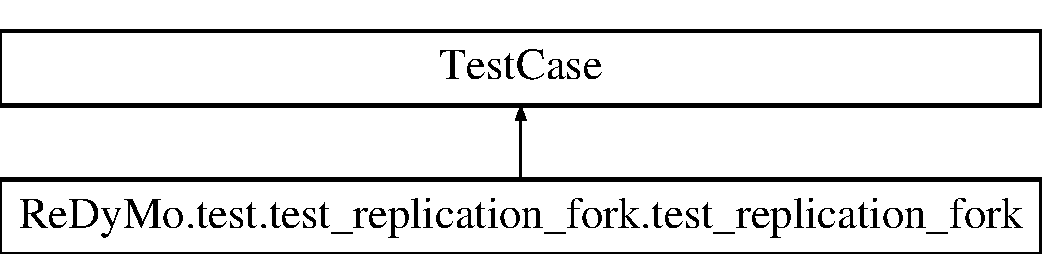
\includegraphics[height=2.000000cm]{classReDyMo_1_1test_1_1test__replication__fork_1_1test__replication__fork}
\end{center}
\end{figure}
\subsection*{Public Member Functions}
\begin{DoxyCompactItemize}
\item 
def \mbox{\hyperlink{classReDyMo_1_1test_1_1test__replication__fork_1_1test__replication__fork_a56e666d191e78294a72a90804a4e70b0}{test\+\_\+constructor}} (self)
\begin{DoxyCompactList}\small\item\em Test the constructor by checking the created object with the input. \end{DoxyCompactList}\item 
def \mbox{\hyperlink{classReDyMo_1_1test_1_1test__replication__fork_1_1test__replication__fork_a318f9d99694530a49fd031659d016e20}{test\+\_\+attach}} (self)
\begin{DoxyCompactList}\small\item\em Test the fork attachment by first trying to attach to an already attached fork, then tries with a non attached for and checks if the replicate method is called with the right parameters. \end{DoxyCompactList}\item 
def \mbox{\hyperlink{classReDyMo_1_1test_1_1test__replication__fork_1_1test__replication__fork_a47ebd7572d932a0ac473c2c4e3b67d43}{test\+\_\+unattach}} (self)
\begin{DoxyCompactList}\small\item\em Test if the fork will reset its variables when it unattaches. \end{DoxyCompactList}\item 
def \mbox{\hyperlink{classReDyMo_1_1test_1_1test__replication__fork_1_1test__replication__fork_a29b0f8fb24e51bb7de864e4fee8da905}{test\+\_\+advance}} (self)
\begin{DoxyCompactList}\small\item\em Test the advancing of the fork by attaching it to a base and checking that the replicate function was called with the right bases. \end{DoxyCompactList}\item 
def \mbox{\hyperlink{classReDyMo_1_1test_1_1test__replication__fork_1_1test__replication__fork_a187dd908541c4bf18642ca5891f05564}{test\+\_\+is\+\_\+attached}} (self)
\begin{DoxyCompactList}\small\item\em Test if a frk will report attached when is and not when it isn\textquotesingle{}t. \end{DoxyCompactList}\end{DoxyCompactItemize}


\subsection{Detailed Description}
This class has tests for each Genomic Location method. 

\begin{DoxySeeAlso}{See also}
Genomic Location 
\end{DoxySeeAlso}


\subsection{Member Function Documentation}
\mbox{\Hypertarget{classReDyMo_1_1test_1_1test__replication__fork_1_1test__replication__fork_a29b0f8fb24e51bb7de864e4fee8da905}\label{classReDyMo_1_1test_1_1test__replication__fork_1_1test__replication__fork_a29b0f8fb24e51bb7de864e4fee8da905}} 
\index{Re\+Dy\+Mo\+::test\+::test\+\_\+replication\+\_\+fork\+::test\+\_\+replication\+\_\+fork@{Re\+Dy\+Mo\+::test\+::test\+\_\+replication\+\_\+fork\+::test\+\_\+replication\+\_\+fork}!test\+\_\+advance@{test\+\_\+advance}}
\index{test\+\_\+advance@{test\+\_\+advance}!Re\+Dy\+Mo\+::test\+::test\+\_\+replication\+\_\+fork\+::test\+\_\+replication\+\_\+fork@{Re\+Dy\+Mo\+::test\+::test\+\_\+replication\+\_\+fork\+::test\+\_\+replication\+\_\+fork}}
\subsubsection{\texorpdfstring{test\+\_\+advance()}{test\_advance()}}
{\footnotesize\ttfamily def Re\+Dy\+Mo.\+test.\+test\+\_\+replication\+\_\+fork.\+test\+\_\+replication\+\_\+fork.\+test\+\_\+advance (\begin{DoxyParamCaption}\item[{}]{self }\end{DoxyParamCaption})}



Test the advancing of the fork by attaching it to a base and checking that the replicate function was called with the right bases. 

\mbox{\Hypertarget{classReDyMo_1_1test_1_1test__replication__fork_1_1test__replication__fork_a318f9d99694530a49fd031659d016e20}\label{classReDyMo_1_1test_1_1test__replication__fork_1_1test__replication__fork_a318f9d99694530a49fd031659d016e20}} 
\index{Re\+Dy\+Mo\+::test\+::test\+\_\+replication\+\_\+fork\+::test\+\_\+replication\+\_\+fork@{Re\+Dy\+Mo\+::test\+::test\+\_\+replication\+\_\+fork\+::test\+\_\+replication\+\_\+fork}!test\+\_\+attach@{test\+\_\+attach}}
\index{test\+\_\+attach@{test\+\_\+attach}!Re\+Dy\+Mo\+::test\+::test\+\_\+replication\+\_\+fork\+::test\+\_\+replication\+\_\+fork@{Re\+Dy\+Mo\+::test\+::test\+\_\+replication\+\_\+fork\+::test\+\_\+replication\+\_\+fork}}
\subsubsection{\texorpdfstring{test\+\_\+attach()}{test\_attach()}}
{\footnotesize\ttfamily def Re\+Dy\+Mo.\+test.\+test\+\_\+replication\+\_\+fork.\+test\+\_\+replication\+\_\+fork.\+test\+\_\+attach (\begin{DoxyParamCaption}\item[{}]{self }\end{DoxyParamCaption})}



Test the fork attachment by first trying to attach to an already attached fork, then tries with a non attached for and checks if the replicate method is called with the right parameters. 

\mbox{\Hypertarget{classReDyMo_1_1test_1_1test__replication__fork_1_1test__replication__fork_a56e666d191e78294a72a90804a4e70b0}\label{classReDyMo_1_1test_1_1test__replication__fork_1_1test__replication__fork_a56e666d191e78294a72a90804a4e70b0}} 
\index{Re\+Dy\+Mo\+::test\+::test\+\_\+replication\+\_\+fork\+::test\+\_\+replication\+\_\+fork@{Re\+Dy\+Mo\+::test\+::test\+\_\+replication\+\_\+fork\+::test\+\_\+replication\+\_\+fork}!test\+\_\+constructor@{test\+\_\+constructor}}
\index{test\+\_\+constructor@{test\+\_\+constructor}!Re\+Dy\+Mo\+::test\+::test\+\_\+replication\+\_\+fork\+::test\+\_\+replication\+\_\+fork@{Re\+Dy\+Mo\+::test\+::test\+\_\+replication\+\_\+fork\+::test\+\_\+replication\+\_\+fork}}
\subsubsection{\texorpdfstring{test\+\_\+constructor()}{test\_constructor()}}
{\footnotesize\ttfamily def Re\+Dy\+Mo.\+test.\+test\+\_\+replication\+\_\+fork.\+test\+\_\+replication\+\_\+fork.\+test\+\_\+constructor (\begin{DoxyParamCaption}\item[{}]{self }\end{DoxyParamCaption})}



Test the constructor by checking the created object with the input. 

\mbox{\Hypertarget{classReDyMo_1_1test_1_1test__replication__fork_1_1test__replication__fork_a187dd908541c4bf18642ca5891f05564}\label{classReDyMo_1_1test_1_1test__replication__fork_1_1test__replication__fork_a187dd908541c4bf18642ca5891f05564}} 
\index{Re\+Dy\+Mo\+::test\+::test\+\_\+replication\+\_\+fork\+::test\+\_\+replication\+\_\+fork@{Re\+Dy\+Mo\+::test\+::test\+\_\+replication\+\_\+fork\+::test\+\_\+replication\+\_\+fork}!test\+\_\+is\+\_\+attached@{test\+\_\+is\+\_\+attached}}
\index{test\+\_\+is\+\_\+attached@{test\+\_\+is\+\_\+attached}!Re\+Dy\+Mo\+::test\+::test\+\_\+replication\+\_\+fork\+::test\+\_\+replication\+\_\+fork@{Re\+Dy\+Mo\+::test\+::test\+\_\+replication\+\_\+fork\+::test\+\_\+replication\+\_\+fork}}
\subsubsection{\texorpdfstring{test\+\_\+is\+\_\+attached()}{test\_is\_attached()}}
{\footnotesize\ttfamily def Re\+Dy\+Mo.\+test.\+test\+\_\+replication\+\_\+fork.\+test\+\_\+replication\+\_\+fork.\+test\+\_\+is\+\_\+attached (\begin{DoxyParamCaption}\item[{}]{self }\end{DoxyParamCaption})}



Test if a frk will report attached when is and not when it isn\textquotesingle{}t. 

\mbox{\Hypertarget{classReDyMo_1_1test_1_1test__replication__fork_1_1test__replication__fork_a47ebd7572d932a0ac473c2c4e3b67d43}\label{classReDyMo_1_1test_1_1test__replication__fork_1_1test__replication__fork_a47ebd7572d932a0ac473c2c4e3b67d43}} 
\index{Re\+Dy\+Mo\+::test\+::test\+\_\+replication\+\_\+fork\+::test\+\_\+replication\+\_\+fork@{Re\+Dy\+Mo\+::test\+::test\+\_\+replication\+\_\+fork\+::test\+\_\+replication\+\_\+fork}!test\+\_\+unattach@{test\+\_\+unattach}}
\index{test\+\_\+unattach@{test\+\_\+unattach}!Re\+Dy\+Mo\+::test\+::test\+\_\+replication\+\_\+fork\+::test\+\_\+replication\+\_\+fork@{Re\+Dy\+Mo\+::test\+::test\+\_\+replication\+\_\+fork\+::test\+\_\+replication\+\_\+fork}}
\subsubsection{\texorpdfstring{test\+\_\+unattach()}{test\_unattach()}}
{\footnotesize\ttfamily def Re\+Dy\+Mo.\+test.\+test\+\_\+replication\+\_\+fork.\+test\+\_\+replication\+\_\+fork.\+test\+\_\+unattach (\begin{DoxyParamCaption}\item[{}]{self }\end{DoxyParamCaption})}



Test if the fork will reset its variables when it unattaches. 



The documentation for this class was generated from the following file\+:\begin{DoxyCompactItemize}
\item 
test/test\+\_\+replication\+\_\+fork.\+py\end{DoxyCompactItemize}

\hypertarget{classReDyMo_1_1test_1_1test__chromosome_1_1TestChromosome}{}\section{Re\+Dy\+Mo.\+test.\+test\+\_\+chromosome.\+Test\+Chromosome Class Reference}
\label{classReDyMo_1_1test_1_1test__chromosome_1_1TestChromosome}\index{Re\+Dy\+Mo.\+test.\+test\+\_\+chromosome.\+Test\+Chromosome@{Re\+Dy\+Mo.\+test.\+test\+\_\+chromosome.\+Test\+Chromosome}}


This class has tests for each Chromosome method.  


Inheritance diagram for Re\+Dy\+Mo.\+test.\+test\+\_\+chromosome.\+Test\+Chromosome\+:\begin{figure}[H]
\begin{center}
\leavevmode
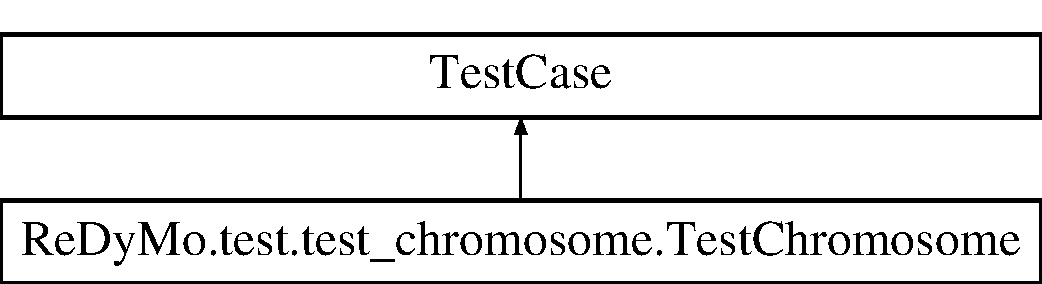
\includegraphics[height=2.000000cm]{classReDyMo_1_1test_1_1test__chromosome_1_1TestChromosome}
\end{center}
\end{figure}
\subsection*{Public Member Functions}
\begin{DoxyCompactItemize}
\item 
def \mbox{\hyperlink{classReDyMo_1_1test_1_1test__chromosome_1_1TestChromosome_a1399201440b0c37de8d1b6fce870f57b}{test\+\_\+constructor}} (self)
\begin{DoxyCompactList}\small\item\em Tests the construction of a Chromosome object. \end{DoxyCompactList}\item 
def \mbox{\hyperlink{classReDyMo_1_1test_1_1test__chromosome_1_1TestChromosome_af729347cc1469bd0043cdba714f4f04c}{test\+\_\+base\+\_\+is\+\_\+replicated}} (self)
\begin{DoxyCompactList}\small\item\em Tests if by changing manually the replicated values the function returns correctly that a base is replicated. \end{DoxyCompactList}\item 
def \mbox{\hyperlink{classReDyMo_1_1test_1_1test__chromosome_1_1TestChromosome_a4a34ea90fad85adb3f9bbb1dbc4753dc}{test\+\_\+is\+\_\+replicated}} (self)
\begin{DoxyCompactList}\small\item\em Tests the function by manually changing the number of replicated bases and checking what the function returns. \end{DoxyCompactList}\item 
def \mbox{\hyperlink{classReDyMo_1_1test_1_1test__chromosome_1_1TestChromosome_a016230d72ebca018818839d90460608c}{test\+\_\+activation\+\_\+probability}} (self)
\begin{DoxyCompactList}\small\item\em Tests by checking if the function return value is the same passed to the constructor. \end{DoxyCompactList}\item 
def \mbox{\hyperlink{classReDyMo_1_1test_1_1test__chromosome_1_1TestChromosome_a22ef06b4ce026761f08ffb7bfca2809a}{test\+\_\+replicate}} (self)
\begin{DoxyCompactList}\small\item\em Tests the replication of a range of bases and checks number of bases replicated. \end{DoxyCompactList}\item 
\mbox{\Hypertarget{classReDyMo_1_1test_1_1test__chromosome_1_1TestChromosome_a7e91e79150e4610a3f019333b8bf322a}\label{classReDyMo_1_1test_1_1test__chromosome_1_1TestChromosome_a7e91e79150e4610a3f019333b8bf322a}} 
def {\bfseries test\+\_\+set\+\_\+dormant\+\_\+origin\+\_\+activation\+\_\+probability} (self)
\end{DoxyCompactItemize}


\subsection{Detailed Description}
This class has tests for each Chromosome method. 

\begin{DoxySeeAlso}{See also}
Chromosome 
\end{DoxySeeAlso}


\subsection{Member Function Documentation}
\mbox{\Hypertarget{classReDyMo_1_1test_1_1test__chromosome_1_1TestChromosome_a016230d72ebca018818839d90460608c}\label{classReDyMo_1_1test_1_1test__chromosome_1_1TestChromosome_a016230d72ebca018818839d90460608c}} 
\index{Re\+Dy\+Mo\+::test\+::test\+\_\+chromosome\+::\+Test\+Chromosome@{Re\+Dy\+Mo\+::test\+::test\+\_\+chromosome\+::\+Test\+Chromosome}!test\+\_\+activation\+\_\+probability@{test\+\_\+activation\+\_\+probability}}
\index{test\+\_\+activation\+\_\+probability@{test\+\_\+activation\+\_\+probability}!Re\+Dy\+Mo\+::test\+::test\+\_\+chromosome\+::\+Test\+Chromosome@{Re\+Dy\+Mo\+::test\+::test\+\_\+chromosome\+::\+Test\+Chromosome}}
\subsubsection{\texorpdfstring{test\+\_\+activation\+\_\+probability()}{test\_activation\_probability()}}
{\footnotesize\ttfamily def Re\+Dy\+Mo.\+test.\+test\+\_\+chromosome.\+Test\+Chromosome.\+test\+\_\+activation\+\_\+probability (\begin{DoxyParamCaption}\item[{}]{self }\end{DoxyParamCaption})}



Tests by checking if the function return value is the same passed to the constructor. 

\mbox{\Hypertarget{classReDyMo_1_1test_1_1test__chromosome_1_1TestChromosome_af729347cc1469bd0043cdba714f4f04c}\label{classReDyMo_1_1test_1_1test__chromosome_1_1TestChromosome_af729347cc1469bd0043cdba714f4f04c}} 
\index{Re\+Dy\+Mo\+::test\+::test\+\_\+chromosome\+::\+Test\+Chromosome@{Re\+Dy\+Mo\+::test\+::test\+\_\+chromosome\+::\+Test\+Chromosome}!test\+\_\+base\+\_\+is\+\_\+replicated@{test\+\_\+base\+\_\+is\+\_\+replicated}}
\index{test\+\_\+base\+\_\+is\+\_\+replicated@{test\+\_\+base\+\_\+is\+\_\+replicated}!Re\+Dy\+Mo\+::test\+::test\+\_\+chromosome\+::\+Test\+Chromosome@{Re\+Dy\+Mo\+::test\+::test\+\_\+chromosome\+::\+Test\+Chromosome}}
\subsubsection{\texorpdfstring{test\+\_\+base\+\_\+is\+\_\+replicated()}{test\_base\_is\_replicated()}}
{\footnotesize\ttfamily def Re\+Dy\+Mo.\+test.\+test\+\_\+chromosome.\+Test\+Chromosome.\+test\+\_\+base\+\_\+is\+\_\+replicated (\begin{DoxyParamCaption}\item[{}]{self }\end{DoxyParamCaption})}



Tests if by changing manually the replicated values the function returns correctly that a base is replicated. 

\mbox{\Hypertarget{classReDyMo_1_1test_1_1test__chromosome_1_1TestChromosome_a1399201440b0c37de8d1b6fce870f57b}\label{classReDyMo_1_1test_1_1test__chromosome_1_1TestChromosome_a1399201440b0c37de8d1b6fce870f57b}} 
\index{Re\+Dy\+Mo\+::test\+::test\+\_\+chromosome\+::\+Test\+Chromosome@{Re\+Dy\+Mo\+::test\+::test\+\_\+chromosome\+::\+Test\+Chromosome}!test\+\_\+constructor@{test\+\_\+constructor}}
\index{test\+\_\+constructor@{test\+\_\+constructor}!Re\+Dy\+Mo\+::test\+::test\+\_\+chromosome\+::\+Test\+Chromosome@{Re\+Dy\+Mo\+::test\+::test\+\_\+chromosome\+::\+Test\+Chromosome}}
\subsubsection{\texorpdfstring{test\+\_\+constructor()}{test\_constructor()}}
{\footnotesize\ttfamily def Re\+Dy\+Mo.\+test.\+test\+\_\+chromosome.\+Test\+Chromosome.\+test\+\_\+constructor (\begin{DoxyParamCaption}\item[{}]{self }\end{DoxyParamCaption})}



Tests the construction of a Chromosome object. 

\mbox{\Hypertarget{classReDyMo_1_1test_1_1test__chromosome_1_1TestChromosome_a4a34ea90fad85adb3f9bbb1dbc4753dc}\label{classReDyMo_1_1test_1_1test__chromosome_1_1TestChromosome_a4a34ea90fad85adb3f9bbb1dbc4753dc}} 
\index{Re\+Dy\+Mo\+::test\+::test\+\_\+chromosome\+::\+Test\+Chromosome@{Re\+Dy\+Mo\+::test\+::test\+\_\+chromosome\+::\+Test\+Chromosome}!test\+\_\+is\+\_\+replicated@{test\+\_\+is\+\_\+replicated}}
\index{test\+\_\+is\+\_\+replicated@{test\+\_\+is\+\_\+replicated}!Re\+Dy\+Mo\+::test\+::test\+\_\+chromosome\+::\+Test\+Chromosome@{Re\+Dy\+Mo\+::test\+::test\+\_\+chromosome\+::\+Test\+Chromosome}}
\subsubsection{\texorpdfstring{test\+\_\+is\+\_\+replicated()}{test\_is\_replicated()}}
{\footnotesize\ttfamily def Re\+Dy\+Mo.\+test.\+test\+\_\+chromosome.\+Test\+Chromosome.\+test\+\_\+is\+\_\+replicated (\begin{DoxyParamCaption}\item[{}]{self }\end{DoxyParamCaption})}



Tests the function by manually changing the number of replicated bases and checking what the function returns. 

\mbox{\Hypertarget{classReDyMo_1_1test_1_1test__chromosome_1_1TestChromosome_a22ef06b4ce026761f08ffb7bfca2809a}\label{classReDyMo_1_1test_1_1test__chromosome_1_1TestChromosome_a22ef06b4ce026761f08ffb7bfca2809a}} 
\index{Re\+Dy\+Mo\+::test\+::test\+\_\+chromosome\+::\+Test\+Chromosome@{Re\+Dy\+Mo\+::test\+::test\+\_\+chromosome\+::\+Test\+Chromosome}!test\+\_\+replicate@{test\+\_\+replicate}}
\index{test\+\_\+replicate@{test\+\_\+replicate}!Re\+Dy\+Mo\+::test\+::test\+\_\+chromosome\+::\+Test\+Chromosome@{Re\+Dy\+Mo\+::test\+::test\+\_\+chromosome\+::\+Test\+Chromosome}}
\subsubsection{\texorpdfstring{test\+\_\+replicate()}{test\_replicate()}}
{\footnotesize\ttfamily def Re\+Dy\+Mo.\+test.\+test\+\_\+chromosome.\+Test\+Chromosome.\+test\+\_\+replicate (\begin{DoxyParamCaption}\item[{}]{self }\end{DoxyParamCaption})}



Tests the replication of a range of bases and checks number of bases replicated. 



The documentation for this class was generated from the following file\+:\begin{DoxyCompactItemize}
\item 
test/test\+\_\+chromosome.\+py\end{DoxyCompactItemize}

\hypertarget{classReDyMo_1_1test_1_1test__genome_1_1TestGenome}{}\section{Re\+Dy\+Mo.\+test.\+test\+\_\+genome.\+Test\+Genome Class Reference}
\label{classReDyMo_1_1test_1_1test__genome_1_1TestGenome}\index{Re\+Dy\+Mo.\+test.\+test\+\_\+genome.\+Test\+Genome@{Re\+Dy\+Mo.\+test.\+test\+\_\+genome.\+Test\+Genome}}


This class has tests for each Genome method.  


Inheritance diagram for Re\+Dy\+Mo.\+test.\+test\+\_\+genome.\+Test\+Genome\+:\begin{figure}[H]
\begin{center}
\leavevmode
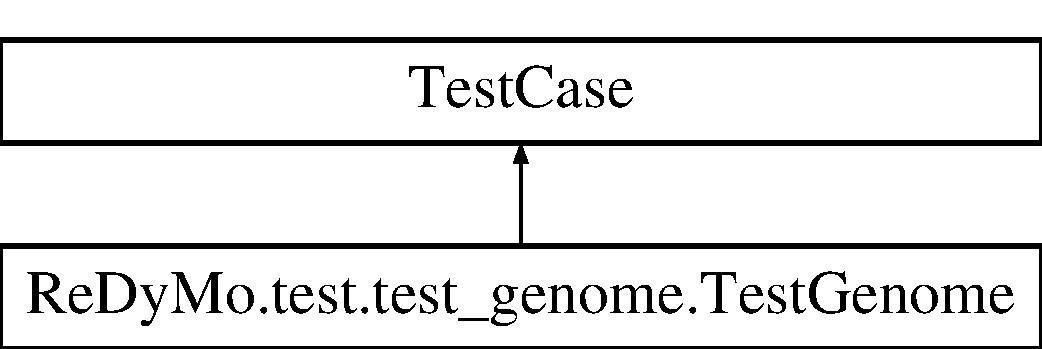
\includegraphics[height=2.000000cm]{classReDyMo_1_1test_1_1test__genome_1_1TestGenome}
\end{center}
\end{figure}
\subsection*{Public Member Functions}
\begin{DoxyCompactItemize}
\item 
\mbox{\Hypertarget{classReDyMo_1_1test_1_1test__genome_1_1TestGenome_ab20586dfa32d303107488319f9012d9a}\label{classReDyMo_1_1test_1_1test__genome_1_1TestGenome_ab20586dfa32d303107488319f9012d9a}} 
def \mbox{\hyperlink{classReDyMo_1_1test_1_1test__genome_1_1TestGenome_ab20586dfa32d303107488319f9012d9a}{test\+\_\+constructor}} (self)
\begin{DoxyCompactList}\small\item\em Tests the constructor by creating a new object and comparing the setted values with the given ones. \end{DoxyCompactList}\item 
def \mbox{\hyperlink{classReDyMo_1_1test_1_1test__genome_1_1TestGenome_a9d1148ac068b11c35cd1d67139b78bfd}{test\+\_\+random\+\_\+genomic\+\_\+location}} (self)
\begin{DoxyCompactList}\small\item\em Tests if the random\+\_\+genomic\+\_\+location stays within the chromosomes\textquotesingle{} area. \end{DoxyCompactList}\item 
def \mbox{\hyperlink{classReDyMo_1_1test_1_1test__genome_1_1TestGenome_aced56bad873a4503b097d17655b0233a}{test\+\_\+is\+\_\+replicated}} (self)
\begin{DoxyCompactList}\small\item\em Tests if the is\+\_\+replicated returns true in true cases and vce versa. \end{DoxyCompactList}\item 
\mbox{\Hypertarget{classReDyMo_1_1test_1_1test__genome_1_1TestGenome_ac5570c5ae42eea415ec9086ae5e2c80e}\label{classReDyMo_1_1test_1_1test__genome_1_1TestGenome_ac5570c5ae42eea415ec9086ae5e2c80e}} 
def \mbox{\hyperlink{classReDyMo_1_1test_1_1test__genome_1_1TestGenome_ac5570c5ae42eea415ec9086ae5e2c80e}{test\+\_\+average\+\_\+interorigin\+\_\+distance}} (self)
\begin{DoxyCompactList}\small\item\em Tests if the function calculates accurately the distance between the origins. \end{DoxyCompactList}\item 
def \mbox{\hyperlink{classReDyMo_1_1test_1_1test__genome_1_1TestGenome_a6a4e2180628fb76e2b44a98870e3df89}{test\+\_\+number\+\_\+of\+\_\+replicated\+\_\+bases\+\_\+in\+\_\+this\+\_\+step}} (self)
\begin{DoxyCompactList}\small\item\em Tests by sending values manually and comparing the returned ones. \end{DoxyCompactList}\end{DoxyCompactItemize}


\subsection{Detailed Description}
This class has tests for each Genome method. 

\begin{DoxySeeAlso}{See also}
Genome 
\end{DoxySeeAlso}


\subsection{Member Function Documentation}
\mbox{\Hypertarget{classReDyMo_1_1test_1_1test__genome_1_1TestGenome_aced56bad873a4503b097d17655b0233a}\label{classReDyMo_1_1test_1_1test__genome_1_1TestGenome_aced56bad873a4503b097d17655b0233a}} 
\index{Re\+Dy\+Mo\+::test\+::test\+\_\+genome\+::\+Test\+Genome@{Re\+Dy\+Mo\+::test\+::test\+\_\+genome\+::\+Test\+Genome}!test\+\_\+is\+\_\+replicated@{test\+\_\+is\+\_\+replicated}}
\index{test\+\_\+is\+\_\+replicated@{test\+\_\+is\+\_\+replicated}!Re\+Dy\+Mo\+::test\+::test\+\_\+genome\+::\+Test\+Genome@{Re\+Dy\+Mo\+::test\+::test\+\_\+genome\+::\+Test\+Genome}}
\subsubsection{\texorpdfstring{test\+\_\+is\+\_\+replicated()}{test\_is\_replicated()}}
{\footnotesize\ttfamily def Re\+Dy\+Mo.\+test.\+test\+\_\+genome.\+Test\+Genome.\+test\+\_\+is\+\_\+replicated (\begin{DoxyParamCaption}\item[{}]{self }\end{DoxyParamCaption})}



Tests if the is\+\_\+replicated returns true in true cases and vce versa. 

\mbox{\Hypertarget{classReDyMo_1_1test_1_1test__genome_1_1TestGenome_a6a4e2180628fb76e2b44a98870e3df89}\label{classReDyMo_1_1test_1_1test__genome_1_1TestGenome_a6a4e2180628fb76e2b44a98870e3df89}} 
\index{Re\+Dy\+Mo\+::test\+::test\+\_\+genome\+::\+Test\+Genome@{Re\+Dy\+Mo\+::test\+::test\+\_\+genome\+::\+Test\+Genome}!test\+\_\+number\+\_\+of\+\_\+replicated\+\_\+bases\+\_\+in\+\_\+this\+\_\+step@{test\+\_\+number\+\_\+of\+\_\+replicated\+\_\+bases\+\_\+in\+\_\+this\+\_\+step}}
\index{test\+\_\+number\+\_\+of\+\_\+replicated\+\_\+bases\+\_\+in\+\_\+this\+\_\+step@{test\+\_\+number\+\_\+of\+\_\+replicated\+\_\+bases\+\_\+in\+\_\+this\+\_\+step}!Re\+Dy\+Mo\+::test\+::test\+\_\+genome\+::\+Test\+Genome@{Re\+Dy\+Mo\+::test\+::test\+\_\+genome\+::\+Test\+Genome}}
\subsubsection{\texorpdfstring{test\+\_\+number\+\_\+of\+\_\+replicated\+\_\+bases\+\_\+in\+\_\+this\+\_\+step()}{test\_number\_of\_replicated\_bases\_in\_this\_step()}}
{\footnotesize\ttfamily def Re\+Dy\+Mo.\+test.\+test\+\_\+genome.\+Test\+Genome.\+test\+\_\+number\+\_\+of\+\_\+replicated\+\_\+bases\+\_\+in\+\_\+this\+\_\+step (\begin{DoxyParamCaption}\item[{}]{self }\end{DoxyParamCaption})}



Tests by sending values manually and comparing the returned ones. 

\mbox{\Hypertarget{classReDyMo_1_1test_1_1test__genome_1_1TestGenome_a9d1148ac068b11c35cd1d67139b78bfd}\label{classReDyMo_1_1test_1_1test__genome_1_1TestGenome_a9d1148ac068b11c35cd1d67139b78bfd}} 
\index{Re\+Dy\+Mo\+::test\+::test\+\_\+genome\+::\+Test\+Genome@{Re\+Dy\+Mo\+::test\+::test\+\_\+genome\+::\+Test\+Genome}!test\+\_\+random\+\_\+genomic\+\_\+location@{test\+\_\+random\+\_\+genomic\+\_\+location}}
\index{test\+\_\+random\+\_\+genomic\+\_\+location@{test\+\_\+random\+\_\+genomic\+\_\+location}!Re\+Dy\+Mo\+::test\+::test\+\_\+genome\+::\+Test\+Genome@{Re\+Dy\+Mo\+::test\+::test\+\_\+genome\+::\+Test\+Genome}}
\subsubsection{\texorpdfstring{test\+\_\+random\+\_\+genomic\+\_\+location()}{test\_random\_genomic\_location()}}
{\footnotesize\ttfamily def Re\+Dy\+Mo.\+test.\+test\+\_\+genome.\+Test\+Genome.\+test\+\_\+random\+\_\+genomic\+\_\+location (\begin{DoxyParamCaption}\item[{}]{self }\end{DoxyParamCaption})}



Tests if the random\+\_\+genomic\+\_\+location stays within the chromosomes\textquotesingle{} area. 



The documentation for this class was generated from the following file\+:\begin{DoxyCompactItemize}
\item 
test/test\+\_\+genome.\+py\end{DoxyCompactItemize}

\hypertarget{classReDyMo_1_1test_1_1test__genomic__location_1_1TestGenomicLocation}{}\section{Re\+Dy\+Mo.\+test.\+test\+\_\+genomic\+\_\+location.\+Test\+Genomic\+Location Class Reference}
\label{classReDyMo_1_1test_1_1test__genomic__location_1_1TestGenomicLocation}\index{Re\+Dy\+Mo.\+test.\+test\+\_\+genomic\+\_\+location.\+Test\+Genomic\+Location@{Re\+Dy\+Mo.\+test.\+test\+\_\+genomic\+\_\+location.\+Test\+Genomic\+Location}}
Inheritance diagram for Re\+Dy\+Mo.\+test.\+test\+\_\+genomic\+\_\+location.\+Test\+Genomic\+Location\+:\begin{figure}[H]
\begin{center}
\leavevmode
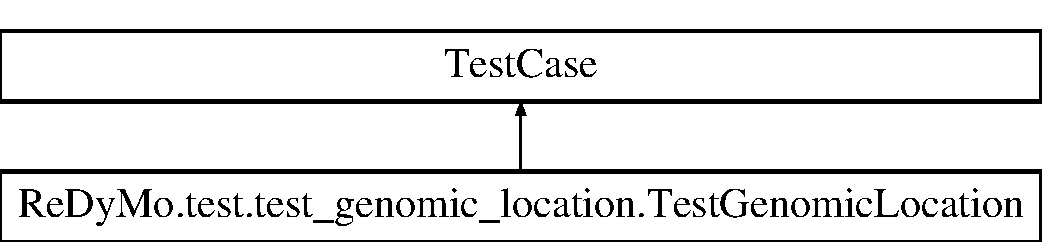
\includegraphics[height=2.000000cm]{classReDyMo_1_1test_1_1test__genomic__location_1_1TestGenomicLocation}
\end{center}
\end{figure}
\subsection*{Public Member Functions}
\begin{DoxyCompactItemize}
\item 
def \mbox{\hyperlink{classReDyMo_1_1test_1_1test__genomic__location_1_1TestGenomicLocation_add11474b7703287f0d310ccb016cfec0}{test\+\_\+constructor}} (self)
\begin{DoxyCompactList}\small\item\em Tests the constructor by comparing the input with the objects generated. \end{DoxyCompactList}\item 
def \mbox{\hyperlink{classReDyMo_1_1test_1_1test__genomic__location_1_1TestGenomicLocation_ada2ce7fa847394f77b6db3f9b1f28445}{test\+\_\+is\+\_\+replicated}} (self)
\begin{DoxyCompactList}\small\item\em Tests by comparing the mock value with the function response. \end{DoxyCompactList}\item 
\mbox{\Hypertarget{classReDyMo_1_1test_1_1test__genomic__location_1_1TestGenomicLocation_a165c828a38385ae5180c0984203207f9}\label{classReDyMo_1_1test_1_1test__genomic__location_1_1TestGenomicLocation_a165c828a38385ae5180c0984203207f9}} 
def \mbox{\hyperlink{classReDyMo_1_1test_1_1test__genomic__location_1_1TestGenomicLocation_a165c828a38385ae5180c0984203207f9}{test\+\_\+will\+\_\+activate}} (self)
\begin{DoxyCompactList}\small\item\em Tests by comaparing. \end{DoxyCompactList}\end{DoxyCompactItemize}


\subsection{Member Function Documentation}
\mbox{\Hypertarget{classReDyMo_1_1test_1_1test__genomic__location_1_1TestGenomicLocation_add11474b7703287f0d310ccb016cfec0}\label{classReDyMo_1_1test_1_1test__genomic__location_1_1TestGenomicLocation_add11474b7703287f0d310ccb016cfec0}} 
\index{Re\+Dy\+Mo\+::test\+::test\+\_\+genomic\+\_\+location\+::\+Test\+Genomic\+Location@{Re\+Dy\+Mo\+::test\+::test\+\_\+genomic\+\_\+location\+::\+Test\+Genomic\+Location}!test\+\_\+constructor@{test\+\_\+constructor}}
\index{test\+\_\+constructor@{test\+\_\+constructor}!Re\+Dy\+Mo\+::test\+::test\+\_\+genomic\+\_\+location\+::\+Test\+Genomic\+Location@{Re\+Dy\+Mo\+::test\+::test\+\_\+genomic\+\_\+location\+::\+Test\+Genomic\+Location}}
\subsubsection{\texorpdfstring{test\+\_\+constructor()}{test\_constructor()}}
{\footnotesize\ttfamily def Re\+Dy\+Mo.\+test.\+test\+\_\+genomic\+\_\+location.\+Test\+Genomic\+Location.\+test\+\_\+constructor (\begin{DoxyParamCaption}\item[{}]{self }\end{DoxyParamCaption})}



Tests the constructor by comparing the input with the objects generated. 

\mbox{\Hypertarget{classReDyMo_1_1test_1_1test__genomic__location_1_1TestGenomicLocation_ada2ce7fa847394f77b6db3f9b1f28445}\label{classReDyMo_1_1test_1_1test__genomic__location_1_1TestGenomicLocation_ada2ce7fa847394f77b6db3f9b1f28445}} 
\index{Re\+Dy\+Mo\+::test\+::test\+\_\+genomic\+\_\+location\+::\+Test\+Genomic\+Location@{Re\+Dy\+Mo\+::test\+::test\+\_\+genomic\+\_\+location\+::\+Test\+Genomic\+Location}!test\+\_\+is\+\_\+replicated@{test\+\_\+is\+\_\+replicated}}
\index{test\+\_\+is\+\_\+replicated@{test\+\_\+is\+\_\+replicated}!Re\+Dy\+Mo\+::test\+::test\+\_\+genomic\+\_\+location\+::\+Test\+Genomic\+Location@{Re\+Dy\+Mo\+::test\+::test\+\_\+genomic\+\_\+location\+::\+Test\+Genomic\+Location}}
\subsubsection{\texorpdfstring{test\+\_\+is\+\_\+replicated()}{test\_is\_replicated()}}
{\footnotesize\ttfamily def Re\+Dy\+Mo.\+test.\+test\+\_\+genomic\+\_\+location.\+Test\+Genomic\+Location.\+test\+\_\+is\+\_\+replicated (\begin{DoxyParamCaption}\item[{}]{self }\end{DoxyParamCaption})}



Tests by comparing the mock value with the function response. 



The documentation for this class was generated from the following file\+:\begin{DoxyCompactItemize}
\item 
test/test\+\_\+genomic\+\_\+location.\+py\end{DoxyCompactItemize}

%--- End generated contents ---

% Index
\backmatter
\newpage
\phantomsection
\clearemptydoublepage
\addcontentsline{toc}{chapter}{Index}
\printindex

\end{document}
